%----------------------------------------------------------------------------------------
%    PACKAGES AND THEMES
%----------------------------------------------------------------------------------------

\documentclass[aspectratio=169,xcolor=dvipsnames]{beamer}

\usetheme{SimplePlus}
\usepackage{graphicx} % Allows including images
\usepackage{booktabs} % Allows the use of \toprule, \midrule and \bottomrule in tables

% % Image compression and optimization settings
% \pdfcompresslevel=9            % Maximum compression for PDF content
% \pdfobjcompresslevel=3         % Compress PDF objects
% \pdfimageresolution=150        % Reduce image resolution to 150 DPI (good for presentations)
% \pdfpkresolution=150           % Font resolution

% % Configure graphicx for better compression
% \DeclareGraphicsExtensions{.pdf,.png,.jpg,.jpeg}
% \graphicspath{{imgs/}{imgs/logos/}{imgs/results/}}

% 



\usepackage[english]{babel}  
\usepackage[utf8]{inputenc}  
\usepackage[T1]{fontenc}
\usepackage{hyperref}
\usepackage{tikz}
\usepackage{fontawesome}
\usetikzlibrary{shapes.geometric, arrows.meta, positioning}

%----------------------------------------------------------------------------------------
%    TITLE PAGE
%----------------------------------------------------------------------------------------

\title{\textbf{DockTDesign}}
\subtitle{\Large Deep Generative Models for \textit{de novo} Drug Design}


\author{Matheus M. P. da Silva}

\institute
{
    PhD in Computational Modeling \\
    Laboratório Nacional de Computação Científica (LNCC/MCTI) \\
    \vspace{0.5em}
    {\faEnvelopeO} \texttt{matheusp@posgrad.lncc.br} \quad {\faGithub} \texttt{\href{https://github.com/mpds}{github.com/mpds}}
    % Your institution for the title page
}
\date{November 6, 2025}

%----------------------------------------------------------------------------------------
%    PRESENTATION SLIDES
%----------------------------------------------------------------------------------------

\begin{document}

\begin{frame}
    % Add logos at the top of the slide
    \begin{center}
        
\includegraphics[height=1.cm]{imgs/logos/logo-instituto-ia.png}
        \hspace{1.cm}
        
\includegraphics[height=1.cm]{imgs/logos/lncc-logo.png}
        \hspace{1.cm}
        
\includegraphics[height=1.cm]{imgs/logos/gmmsb-logo.png}
    \end{center}
    \vspace{-5em}

    % print the title page as the first slide
    \titlepage
\end{frame}

\begin{frame}{Summary}

    \tableofcontents
    % \begin{columns}[c]
    %     \column{.6\textwidth} % Left column for table of contents
    %     \column{.25\textwidth} % Right column for QR code and link
    %     \begin{center}
    %         \begin{figure}
    %             \centering
    %             
\includegraphics[width=0.6\linewidth]{imgs/qrcode-alt.pdf}
    %         \end{figure}
    %         \vspace{0.3em}
    %         {\color{blue} \underline{\footnotesize{{\href{https://bit.ly/slides-defesa-matheus}{bit.ly/slides-defesa-matheus}}}}}
    %     \end{center}
    % \end{columns}
\end{frame}





%%%%%%%%%%%%%%%%%%%%%%%%%%%%%%%%%%%%%%%%%%
\section{Introduction and Motivation}


\begin{frame}{Motivation}
    % \framesubtitle{The challenge of drug development}
    \begin{columns}[c]

        \column{.45\textwidth} % Left column and width
        \begin{figure}
            \centering
            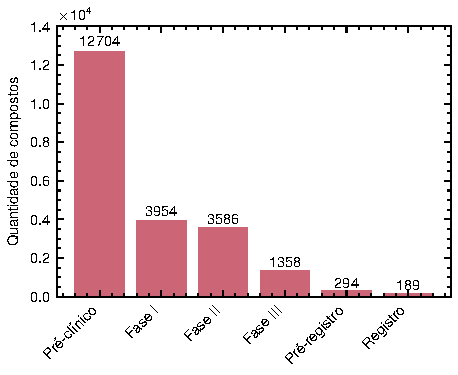
\includegraphics[width=1\linewidth]{imgs/pipeline-sizes.pdf}
            \caption{Number of compounds per development phase in 2025. Source: {\color{blue} \underline{\href{https://www.citeline.com/-/media/C28F0B5022334A4EAC9B0DDDE55F5737}{Pharmaprojects}}.}}
        \end{figure}

        \column{.45\textwidth} % Right column and width
        \begin{itemize}
            \item Drug development: long, costly, and with low success rates ($\leq$ 5\% in the preclinical phase).
                  % \item In 2025, more than 12,700 compounds were in the preclinical phase.
            \item Increasing the success rate in early phases can have a large economic and public-health impact.
            \item Computational methods are essential for the early identification of promising molecules (\textit{hits}).
        \end{itemize}
    \end{columns}
\end{frame}



% \begin{frame}{IA\footnote{inteligência artificial.} na descoberta de fármacos}
%     \begin{columns}[c]
%         \column{.55\textwidth}
%         \begin{figure}
%             \centering
%             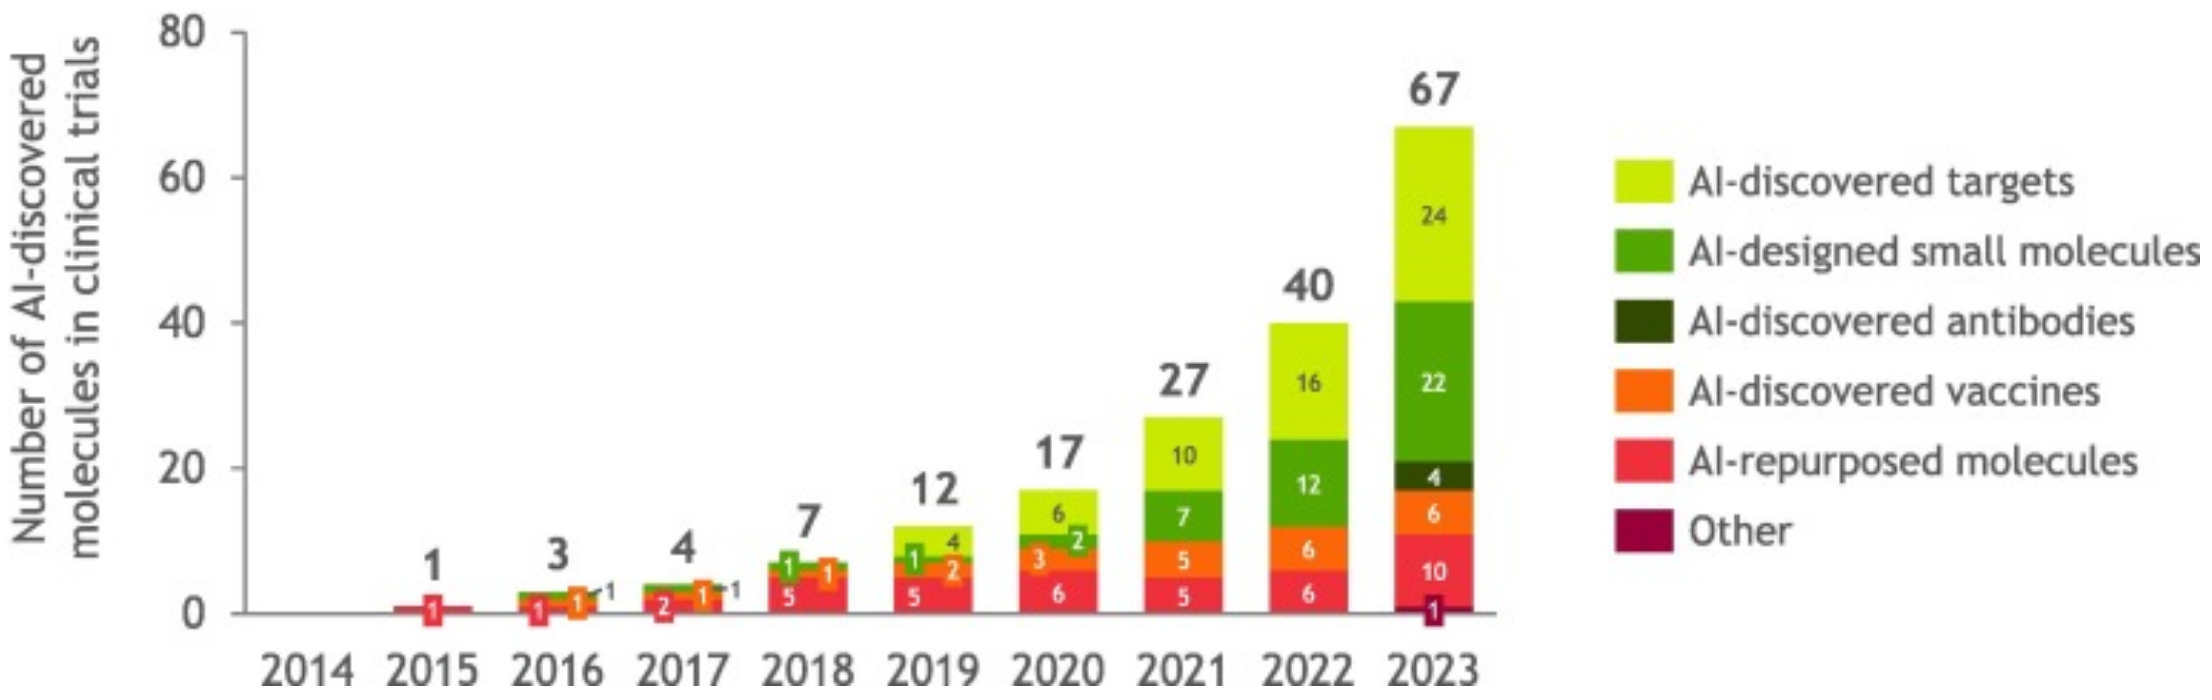
\includegraphics[width=1\linewidth]{imgs/ai-discovered-drugs.png}
%             \caption{Quantidade de moléculas descobertas com auxílio de IA que entraram em ensaios clínicos.~\cite{jayatunga2024successful}}
%         \end{figure}
%         \column{.35\textwidth}
%         \begin{itemize}
%             \item Moléculas descobertas por IA têm taxa de sucesso de 80-90\% na fase 1.
%             \item O uso de IA tem o potencial de dobrar a porcentagem de moléculas aprovadas na fase 3 nos próximos anos.
%         \end{itemize}
%     \end{columns}
% \end{frame}


\begin{frame}{Identification of \textit{hits} \hfill Receptor-ligand docking}
    \begin{columns}[c]
        \column{.45\textwidth}
        \begin{block}{Objectives}
            \begin{itemize}
                \item Pose prediction
                \item Binding affinity prediction
            \end{itemize}
        \end{block}

        \begin{block}{Components}
            \begin{itemize}
                \item Search algorithm
                \item Scoring function:
                      \begin{itemize}
                          \item pose
                          \item binding affinity
                      \end{itemize}
            \end{itemize}

        \end{block}
        \column{.45\textwidth}

        \begin{figure}
            \centering
            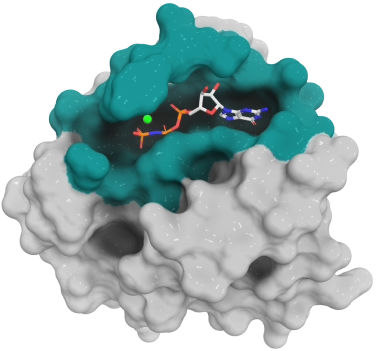
\includegraphics[width=.8\linewidth]{imgs/docking.png}
            % \caption{Receptor-ligand docking.}
        \end{figure}

    \end{columns}
\end{frame}


% \begin{frame}{Hit identification \hfill {\normalsize ML-based scoring functions\footnote{machine learning (\textit{machine learning}).}}}
%     \begin{columns}[c]
%         \column{.45\textwidth}
%         \begin{figure}
%             \centering
%             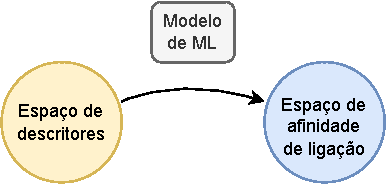
\includegraphics[width=.81\linewidth]{imgs/mlsf.pdf}
%             \caption{Scoring functions based on machine learning techniques (MLSFs).}
%         \end{figure}

%         \column{.45\textwidth}
%         \begin{itemize}
%             \item Seek to reproduce experimental binding affinity values.
%             \item Predictions based on a single pose of the receptor-ligand complex.
%             \item Use datasets with structural and affinity information in their construction.
%         \end{itemize}
%     \end{columns}
% \end{frame}



\begin{frame}{Hit identification \hfill Virtual screening}
    \begin{columns}[c]
        \column{.45\textwidth}
        \begin{itemize}
            \item Identify \textit{hits} with high binding affinity from large virtual compound libraries.
                  % \item \alert{Fast and accurate scoring functions are essential.}
        \end{itemize}

        \column{.45\textwidth}
        \begin{figure}
            \centering
            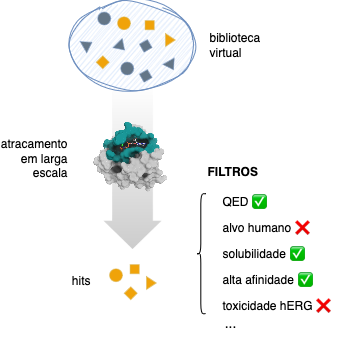
\includegraphics[width=0.95\linewidth]{imgs/virtual-screening.png}
            % \caption{Virtual screening of compounds.}
        \end{figure}
    \end{columns}
\end{frame}



\begin{frame}{Hit identification \hfill \textit{De novo} molecule design}
    \begin{columns}[c]
        \column{.35\textwidth}
        \begin{itemize}
            \item Generate molecules with desirable properties without the need for pre-defined structures and fixed databases.
            \item Essentially multi-objective problem.
                  % \item \alert{Fast and accurate scoring functions are essential.}
        \end{itemize}

        \column{.55\textwidth}
        \begin{figure}
            \centering
            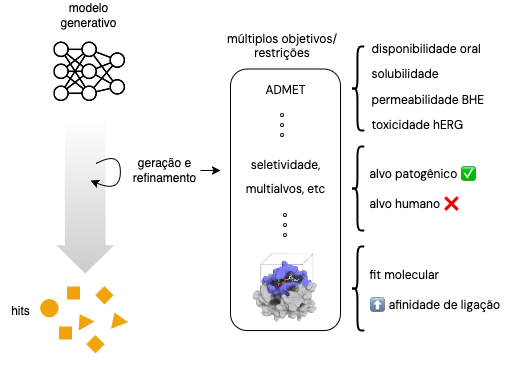
\includegraphics[width=.99\linewidth]{imgs/desenho-denovo.png}
        \end{figure}

    \end{columns}
\end{frame}


% \subsection{Objetivo geral}


% \begin{frame}{Thesis objectives}
%     \begin{block}{General objective}
%         Development of methodologies based on artificial intelligence (AI) for hit discovery, focusing on:
%         \begin{itemize}
%             \item[1.] prediction of receptor-ligand affinity via 3D convolutional neural networks;
%             \item[2.] \textit{de novo} generation of molecules using generative ML models and \textit{many}-objective evolutionary algorithms.
%         \end{itemize}
%     \end{block}
% \end{frame}


% \section{Fundamentação Teórica}

% \begin{frame}  % transition page
%     \Large{\centerline{\textbf{Theoretical Foundation}}}
% \end{frame}

\subsection{Machine Learning and Deep Learning}
\begin{frame}{Machine Learning}
    Machine learning consists of:
    \begin{itemize}
        \item[1.] obtaining a representative dataset of the problem of interest;
        \item[2.] constructing a statistical model based on the dataset (training).
    \end{itemize}

    \begin{columns}[c]
        \column{.45\textwidth}
        % Paradigmas de aprendizado:
        % \begin{itemize}
        %     \item supervisionado;
        %     \item não~supervisionado;
        %     \item por reforço.
        % \end{itemize}
        {\small
            \textbf{Supervised learning}:
            \begin{align*}
                \mathcal{D} & = \{(x_i, y_i)\}_{i=1}^n,                                                 \\
                f^*         & = \arg\min_{f \in \mathcal{F}} \; \mathbb{E}_{(x,y)\sim P}[\ell(f(x),y)].
            \end{align*}

            \textbf{Unsupervised learning}:
            \begin{align*}
                \mathcal{D}' & = \{x_i\}_{i=1}^n,                                                  \\
                h^*          & = \arg\min_{h \in \mathcal{H}} \; \mathbb{E}_{x\sim P}[\ell(h(x))].
            \end{align*}
        }

        \column{.475\textwidth}
        \begin{figure}
            \centering
            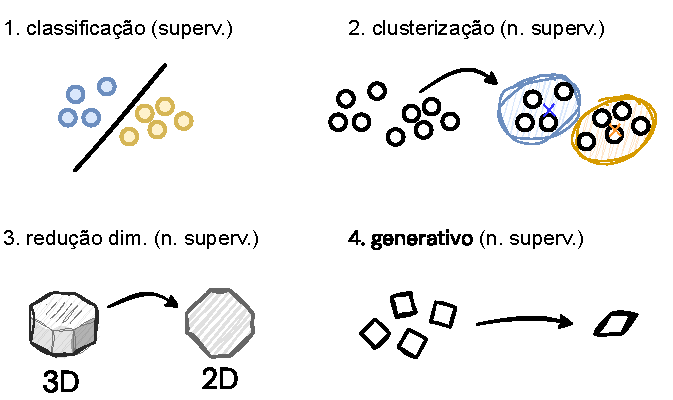
\includegraphics[width=1\textwidth]{imgs/leaning-tasks.pdf}
            \caption{Learning tasks.}
        \end{figure}



    \end{columns}
\end{frame}


% \begin{frame}{Deep Learning}
%     \begin{columns}[c]
%         \column{.45\textwidth}
%         % \begin{itemize}
%         %     \item Aprendizado profundo refere-se a modelos de ML com múltiplas camadas de transformações:
%         % \end{itemize}
%         Deep learning refers to ML models with multiple layers of transformations:
%         \begin{equation*}
%             f_\theta(x) = f^{(L)}_{\theta_L} \circ f^{(L-1)}_{\theta_{L-1}} \circ \dots \circ f^{(1)}_{\theta_1}(x).
%         \end{equation*}

%         \vspace{1.5em}

%         Computation performed by a neuron:
%         \begin{equation*}
%             a = g(w^\top x + b),
%         \end{equation*}
%         where $g(\cdot)$ is a non-linear activation function, $w \in \mathbb{R}^m$ are the weights, $b \in \mathbb{R}$ is the bias, and $x \in \mathbb{R}^m$ is the input.

%         \column{.45\textwidth}

%         \begin{figure}
%             \centering
%             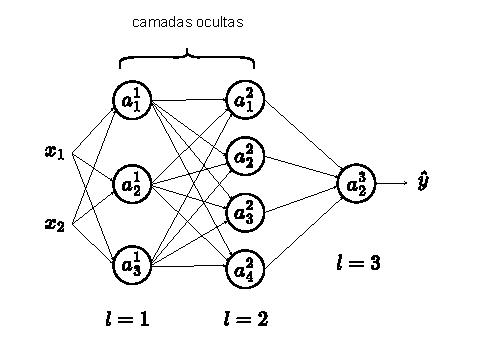
\includegraphics[width=1.\linewidth]{imgs/mlp.pdf}
%             \caption{Architecture of an artificial neural network.}
%         \end{figure}

%     \end{columns}
% \end{frame}



% \begin{frame}{Convolutional Neural Networks (CNNs)}

%     \begin{columns}[t]
%         \column{.55\textwidth}
%         \begin{itemize}
%             \item Local receptive fields.
%             \item Weight sharing.
%             \item Learning hierarchical representations.
%         \end{itemize}
%         %
%         \begin{figure}
%             \centering
%             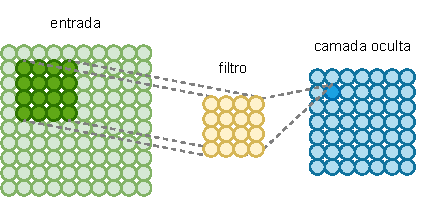
\includegraphics[width=1\linewidth]{imgs/convolution.pdf}
%             \caption{Convolution operation ($X \ast F = Z$).}
%         \end{figure}

%         \column{.35\textwidth}
%         \begin{figure}
%             \centering
%             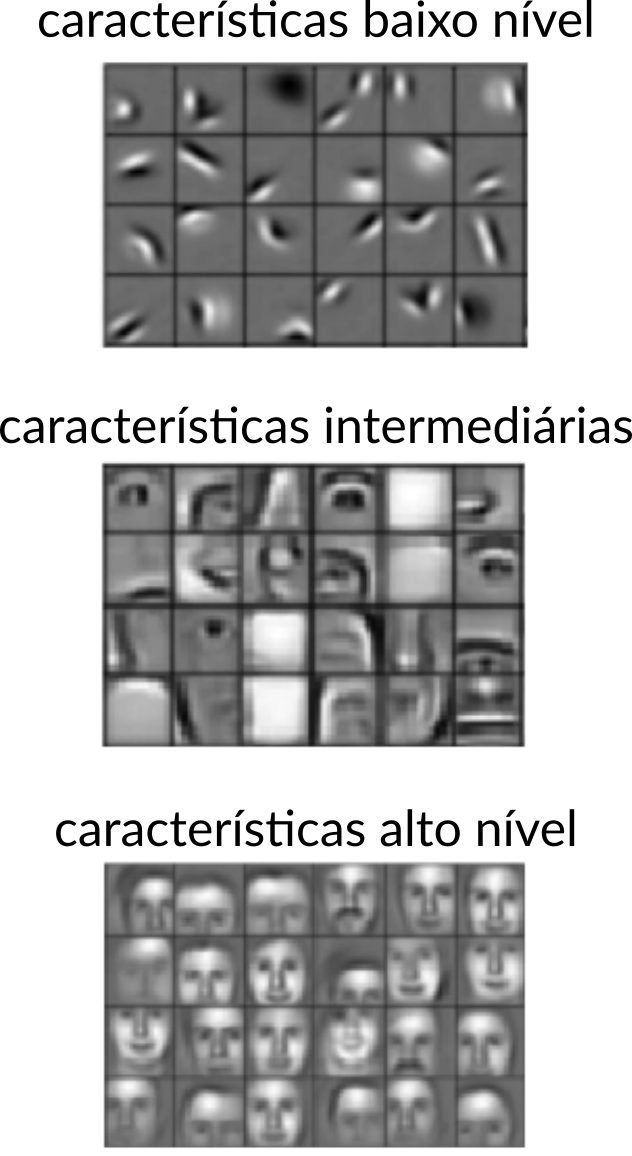
\includegraphics[width=.6\linewidth]{imgs/hierarchical.png}
%             \caption{Hierarchical representations.}
%         \end{figure}
%     \end{columns}
% \end{frame}


% TALVEZ COLOCAR ESTE SLIDE NOS EXTRAS
% \begin{frame}{Redes neurais em grafos (GNNs)}
%     \begin{columns}[t]
%         \column{.45\textwidth}
%         \begin{itemize}
%             \item Dados estruturados como grafos (representação não euclidiana).
%             \item Passagem de mensagens entre os nós do grafo.
%             \item Invariante/equivariante a permutações.
%         \end{itemize}

%         \vspace{1em}
%         Camada de convolução em grafos:
%         \begin{equation*}
%             h_v' = g \left( W \cdot \sum_{u \in \mathcal{N}_v \cup \{v\}} \frac{1}{\sqrt{|\mathcal{N}_v||\mathcal{N}_u|}} \, h_u \right).
%         \end{equation*}

%         \column{.45\textwidth}
%         \begin{figure}
%             \centering
%             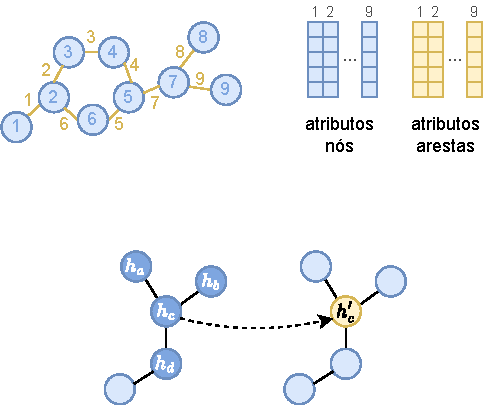
\includegraphics[width=1\linewidth]{imgs/gnn.pdf}
%             \caption{GNNs e passagem de mensagem.}
%         \end{figure}
%     \end{columns}
% \end{frame}

\begin{frame}{Variational Autoencoders (VAEs)}
    \begin{itemize}
        % \item Modelos generativos visam capturar a estrutura subjacente dos dados em um espaço latente.
        \item VAEs learn a \alert{continuous} and \alert{regular} latent space by modeling latent variables as probabilistic distributions.
        \item Latent space acquires ``semantics'', favoring interpretation, manipulation, and robustness.
    \end{itemize}
    \vspace{-1em}
    \begin{columns}[t]
        \column{.55\textwidth}
        \begin{figure}
            \centering
            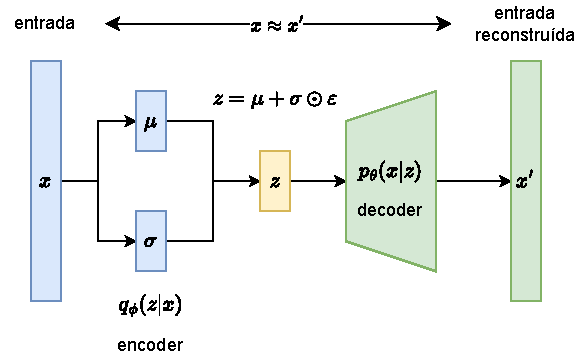
\includegraphics[width=0.8\linewidth]{imgs/vae.pdf}
            \caption{Variational Autoencoder (VAE).}
        \end{figure}

        \column{.475\textwidth}
        \begin{figure}
            \centering
            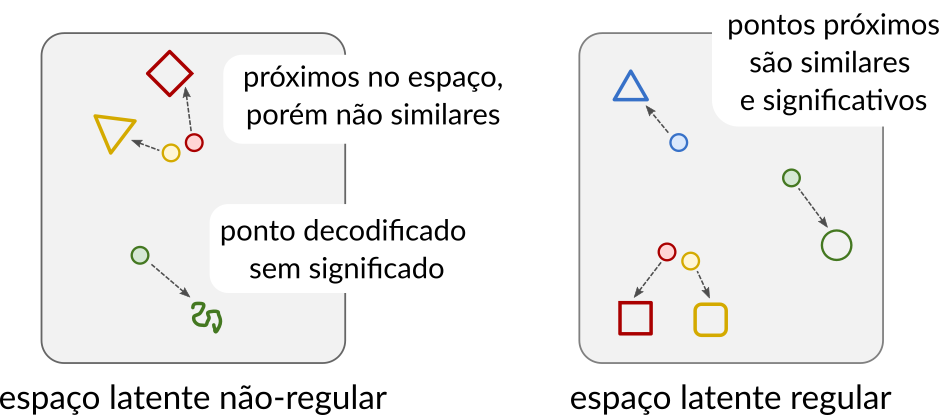
\includegraphics[width=0.9\linewidth]{imgs/latent-space-properties.png}
            \caption{Properties of the latent space.}
        \end{figure}

    \end{columns}
\end{frame}




% \subsubsection{Autoencoders Variacionais}
\subsection{Multi and \textit{Many}-Objective Optimization}
% \subsubsection{Além de três objetivos: otimização \textit{many}-objetivo}

% \begin{frame}{Otimização mono-objetivo}
%     \begin{columns}[c]
%         \column{.45\textwidth}
%         % Otimização mono-objetivo:
%         \begin{equation*}
%             \begin{aligned}
%                  & \text{minimizar}       &  & f(x) \in \mathbb{R}, &  & x = (x_1, \ldots, x_n)^T \\
%                  & \text{sujeito a} \quad &  & g_i(x) \leq 0,       &  & i = 1, \dots, m          \\
%                  &                        &  & h_j(x) = 0,          &  & j = 1, \dots, p          \\
%                 %  &                        &  & x \in \Omega
%             \end{aligned}
%         \end{equation*}

%         \column{.45\textwidth}
%         \begin{figure}
%             \centering
%             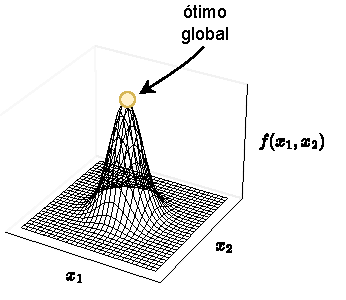
\includegraphics[width=0.8\linewidth]{imgs/global-optim.pdf}
%             \caption{Função objetivo com um ótimo global.}
%         \end{figure}

%     \end{columns}
% \end{frame}

\begin{frame}{Multi-objective optimization}
    \begin{columns}[c]
        \column{.5\textwidth}
        \begin{equation*}
            \begin{aligned}
                \text{minimize }   & \quad F(x) = (f_1(x), f_2(x), \dots, f_k(x))^T \\
                \text{subject to } & \quad g_i(x) \leq 0, \quad i = 1, 2, \dots, m  \\
                                   & \quad h_j(x) = 0, \quad j = 1, 2, \dots, p     \\
                %   & \quad x \in \Omega.
            \end{aligned}
        \end{equation*}
        $f_i: \mathbb{R}^n \rightarrow \mathbb{R}$

        \vspace{1em}
        % A maneira mais intuitiva de resolver um problema multi-objetivo é convertê-lo em um problema mono-objetivo:
        \begin{block}{Intuitive resolution}
            Convert to single-objective problem via weighted sum:
            \vspace{-.85em}
            \begin{align*}
                \text{min } & \sum_{i=1}^k w_i f_i(x), \quad \sum_{i=1}^k w_i = 1, \; w_i \geq 0.
            \end{align*}
        \end{block}



        \column{.4\textwidth}
        \begin{figure}
            \centering
            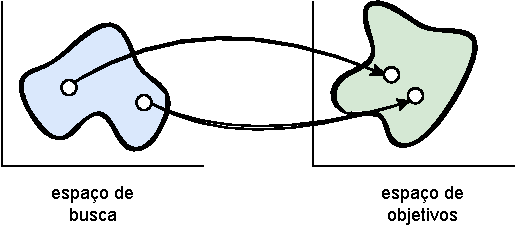
\includegraphics[width=1\linewidth]{imgs/objective-space.pdf}
            \caption{Different spaces in multi-objective optimization.}
        \end{figure}

        Objective space: $F(x) = z = (z_1, z_2,\dots,z_k)^T$, where $z_i = f_i$.

    \end{columns}
\end{frame}


\begin{frame}{Dominance and Pareto Front}
    \begin{columns}[c]
        \column{.45\textwidth}
        % A dominância é uma relação entre soluções em um espaço de objetivos. Uma solução $x_1$ é dita dominar outra solução $x_2$ se:
        We say that $x_1$ dominates $x_2$ if:
        \begin{itemize}
            \item $f_i(x_1) \leq f_i(x_2)$ for all $i$ (i.e., $x_1$ is better or equal in all objectives)
            \item $f_j(x_1) < f_j(x_2)$ for at least one $j$ (i.e., $x_1$ is strictly better in at least one objective)
        \end{itemize}
        \vspace{1em}
        In multi-objective optimization, we seek solutions as close as possible to the Pareto front (\alert{convergence}) and as diverse as possible along it (\alert{diversity}).

        \column{.45\textwidth}
        \begin{figure}
            \centering
            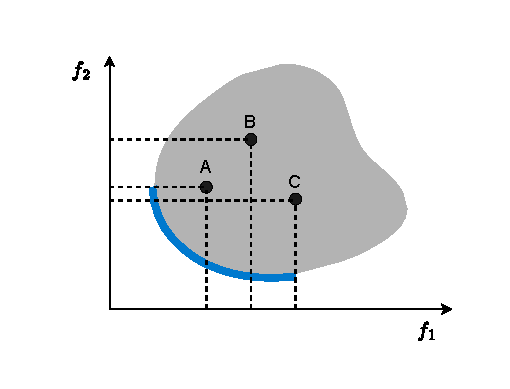
\includegraphics[width=1.0\linewidth]{imgs/pareto-front.pdf}
            \caption{Pareto Front.}
        \end{figure}
    \end{columns}
\end{frame}



\begin{frame}{\textit{Many}-objective optimization}
    Problems with optimization with $k > 3$ objectives are called \textit{many}-objective and present additional challenges:
    \begin{itemize}
        \item Curse of dimensionality: the volume of the search space grows exponentially with $k$.
        \item Dominance resistance: most solutions tend to be non-dominated.
        \item Visualization of solutions: difficult to represent and interpret.
    \end{itemize}

    \vspace{1em}
    % Dessa forma, problemas \textit{many}-objetivo usualmente requerem algoritmos especializados para lidar com esses desafios.
    \begin{block}{State of the art}
        Specific techniques for multi-objective optimization maintain the objective functions separate. Examples include evolutionary algorithms, such as \alert{NSGA-II} and \alert{NSGA-III}.
    \end{block}
\end{frame}



% \begin{frame}{Resolvendo problemas de otimização multi e \textit{many}-objetivo}


%     A resolução de problemas multi-objetivo geralmente envolve três etapas principais:
%     \begin{itemize}
%         \item[1.] \textbf{modelagem}, no qual defini-se os objetivos e restrições do problema;
%         \item[2.] \textbf{otimização}, na qual se aplica uma técnica para obter soluções;
%         \item[3.] \textbf{tomada de decisão}, em que um tomador de decisão seleciona a(s) solução(ões) mais adequada(s).
%     \end{itemize}

% \end{frame}


% \section{Literature Review}

% % transtion page 
% \begin{frame}  % transition page
%     \Large{\centerline{\textbf{Literature Review}}}
% \end{frame}



% \begin{frame}{Literature Review: MLSFs \hfill {\footnotesize \alert{DockTDeep}}}
%     \begin{columns}
%         \column{.45\textwidth}
%         MLSFs\footnote{machine learning-based scoring functions (MLSFs).} show \alert{superior performance} to classical functions in various benchmarks.

%         \column{.45\textwidth}
%         \begin{figure}
%             \centering
%             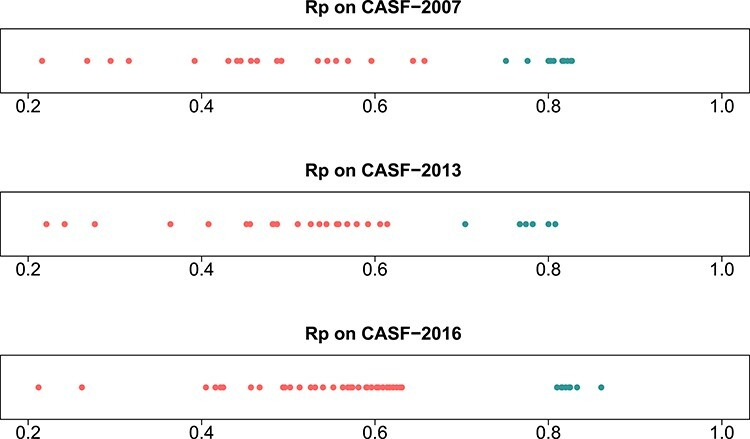
\includegraphics[width=1.\linewidth]{imgs/performance-classical-vs-mlsf.jpg}
%             \caption{Comparative performance between classical functions (red) and MLSFs (green)~\cite{li2021machine}.}
%         \end{figure}
%     \end{columns}
% \end{frame}



% \begin{frame}{Literature Review: MLSFs \hfill {\footnotesize \alert{DockTDeep}}}
%     \begin{columns}[t]
%         \column{.395\textwidth}
%         \begin{itemize}
%             \item Doubts about the learning of intermolecular interactions and the real \alert{generalization capacity} for new targets and ligands.
%             \item ``Out-of-domain'' datasets have emerged as a more challenging evaluation.
%             \item Strategies proposed to mitigate these biases: \textit{docking}, \textit{decoys}, and \textit{crossdocking}.
%         \end{itemize}

%         \column{.55\textwidth}
%         \vspace{-1em}
%         \begin{figure}
%             \centering
%             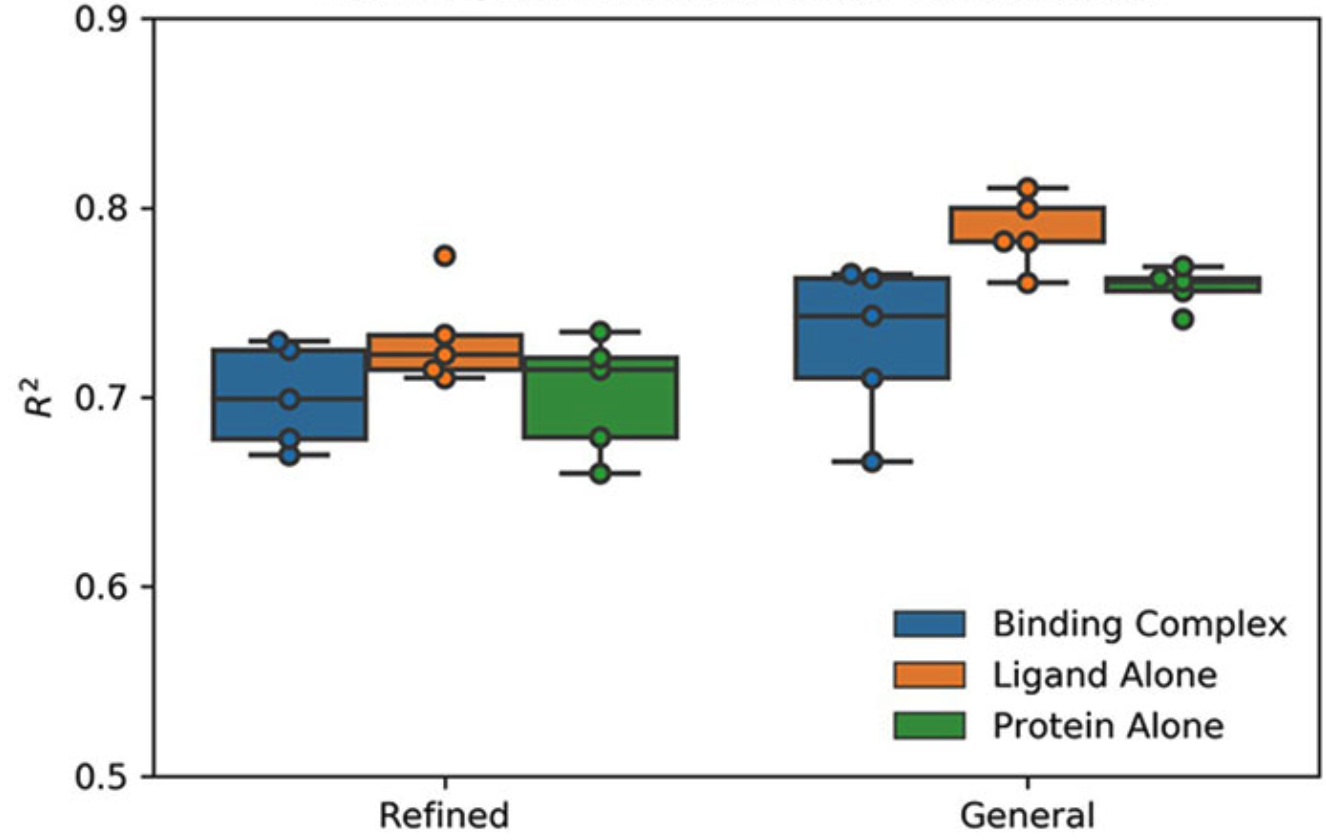
\includegraphics[width=0.5\linewidth]{imgs/protein-ligand-bias.png}
%             \vspace{-0.5em}
%             \caption{Ligand and protein bias~\cite{yang2020predicting}.}
%         \end{figure}
%         \vspace{-1em}
%         \begin{figure}
%             \centering
%             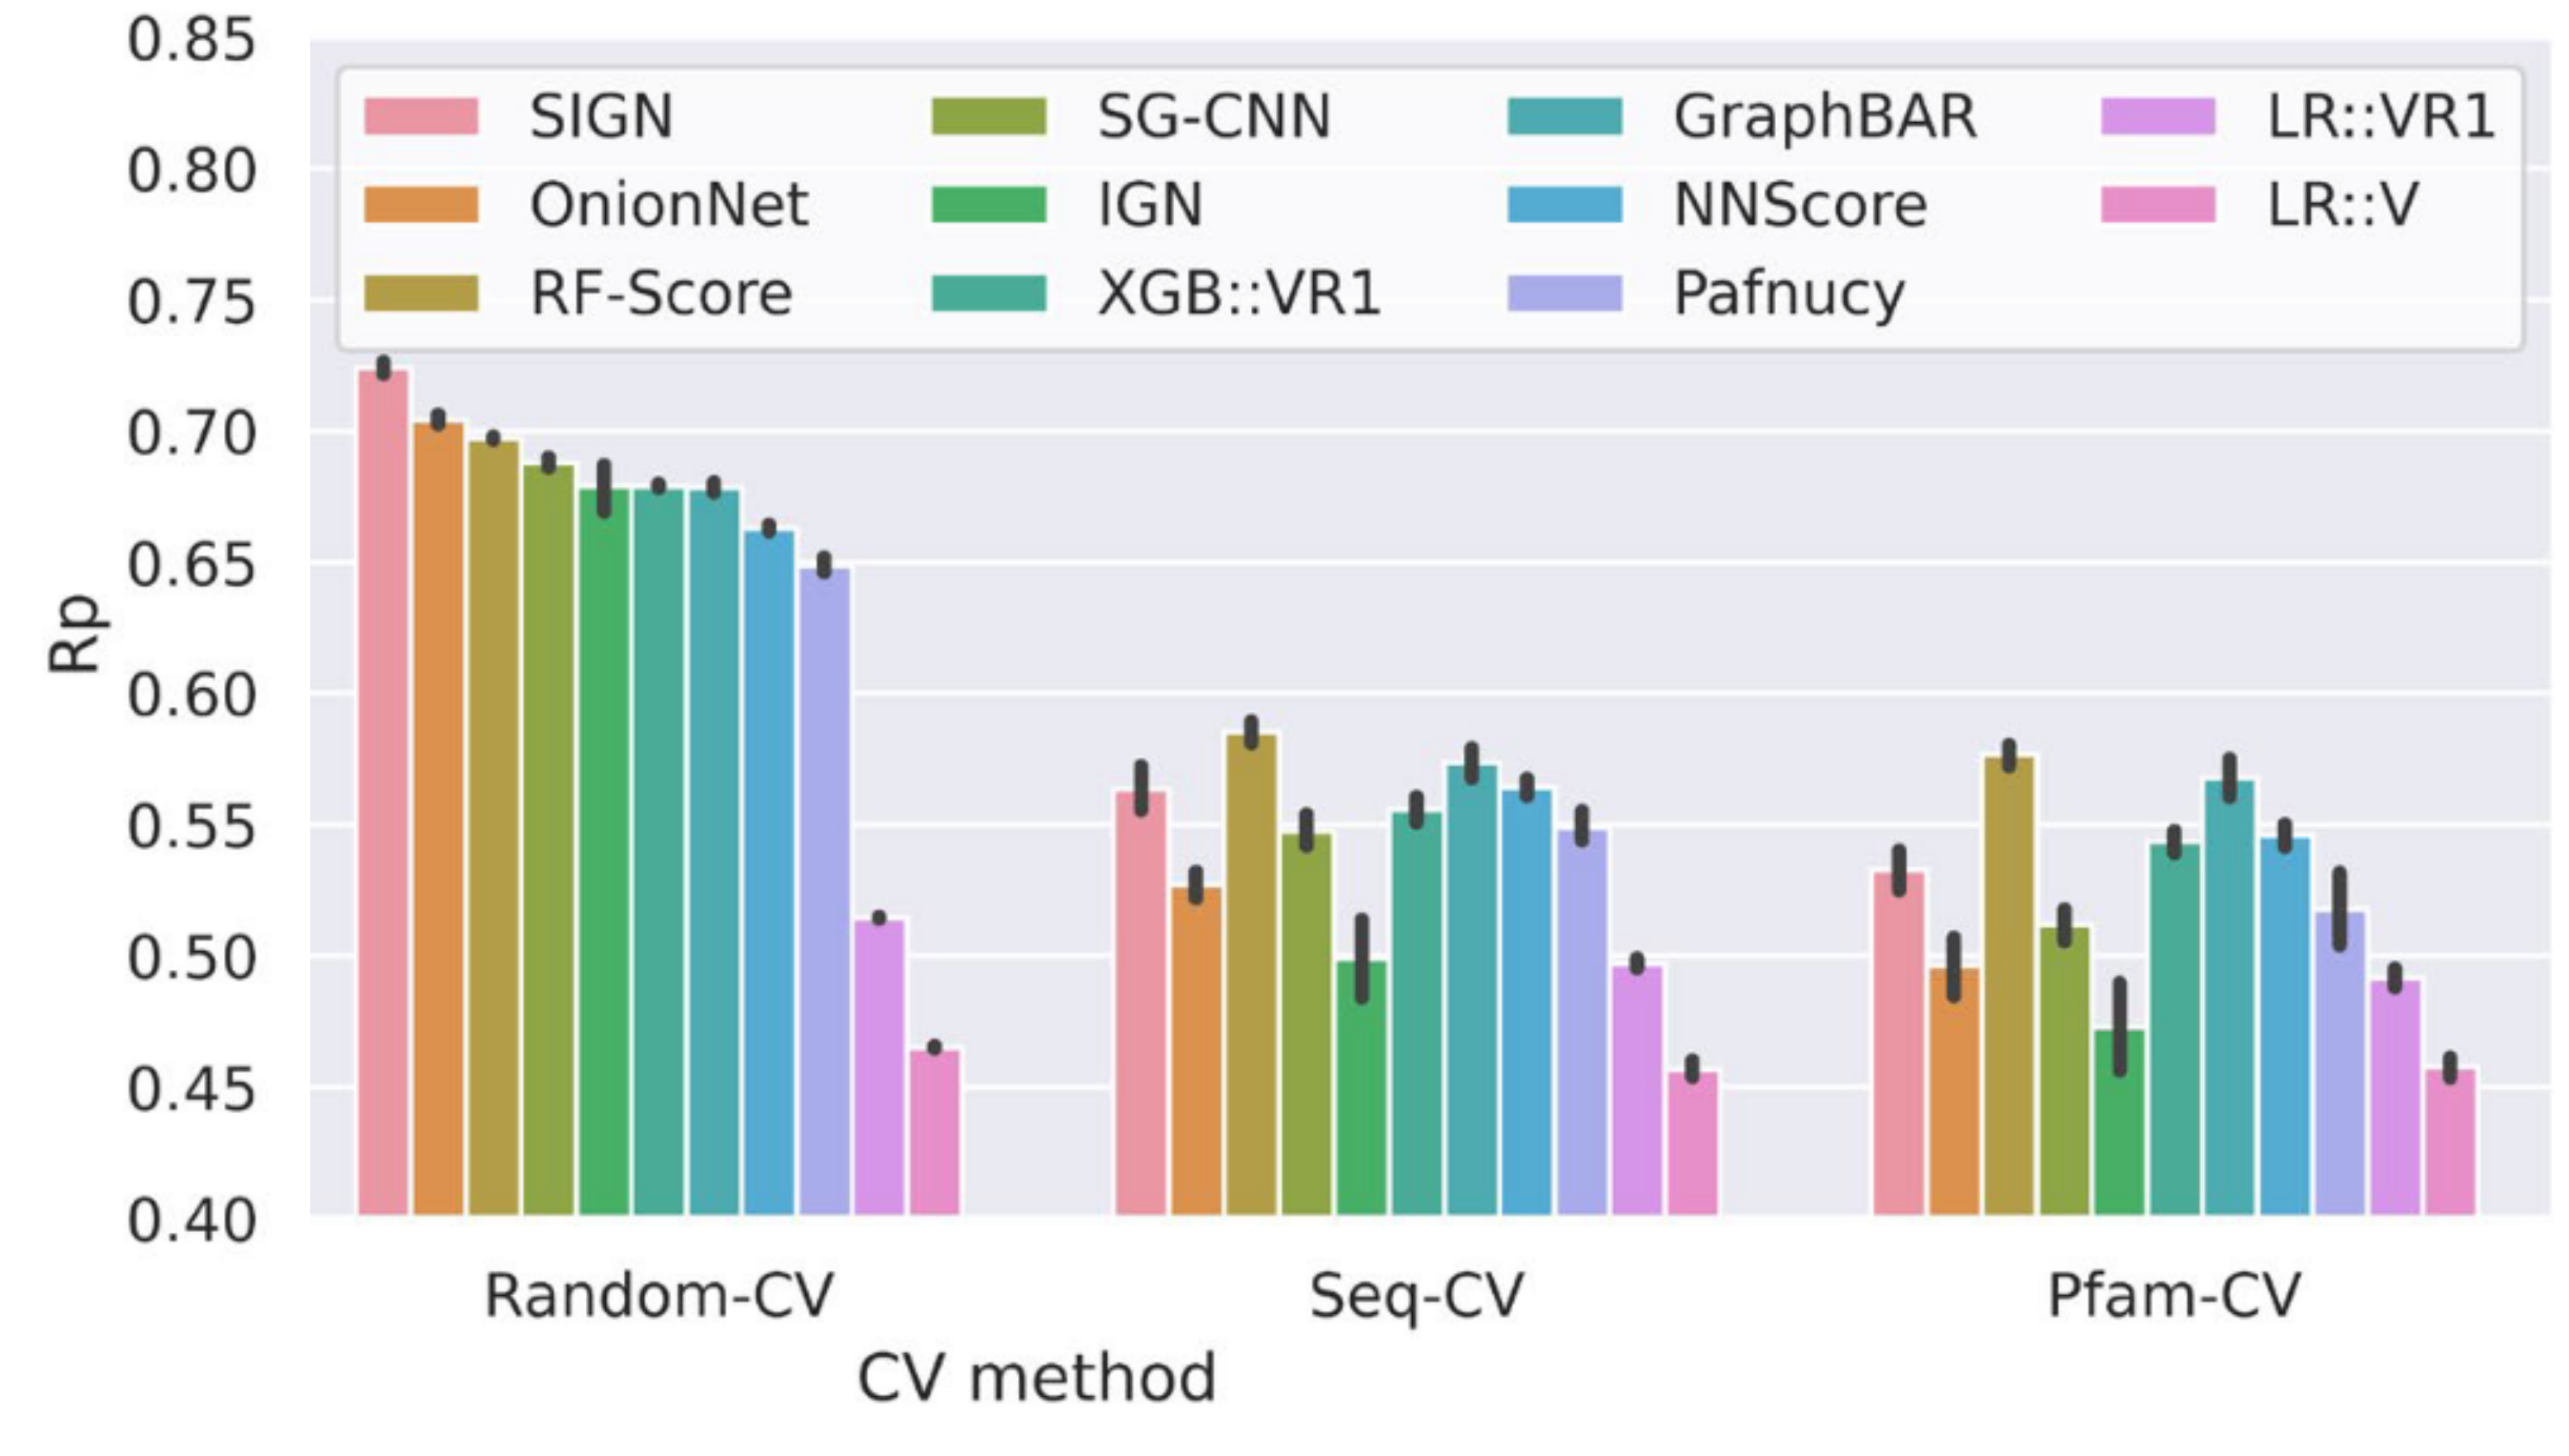
\includegraphics[width=0.6\linewidth]{imgs/pfam-cv.png}
%             \vspace{-0.5em}
%             \caption{Performance on out-of-domain sets~\cite{zhu2022assessment}.}
%         \end{figure}

%     \end{columns}
% \end{frame}

% \begin{frame}{Literature Review: MLSFs \hfill {\footnotesize \alert{DockTDeep}}}

%     \begin{columns}
%         \column{.45\textwidth}
%         \begin{itemize}
%             \item CNNs are not \alert{rotation invariant}.
%             \item Two data augmentation approaches~\cite{da2025data}:
%                   \begin{itemize}
%                       \item 90° rotations (widely used);
%                       \item random rotations in the complex.
%                   \end{itemize}
%         \end{itemize}

%         \column{.45\textwidth}
%         \begin{figure}
%             \centering
%             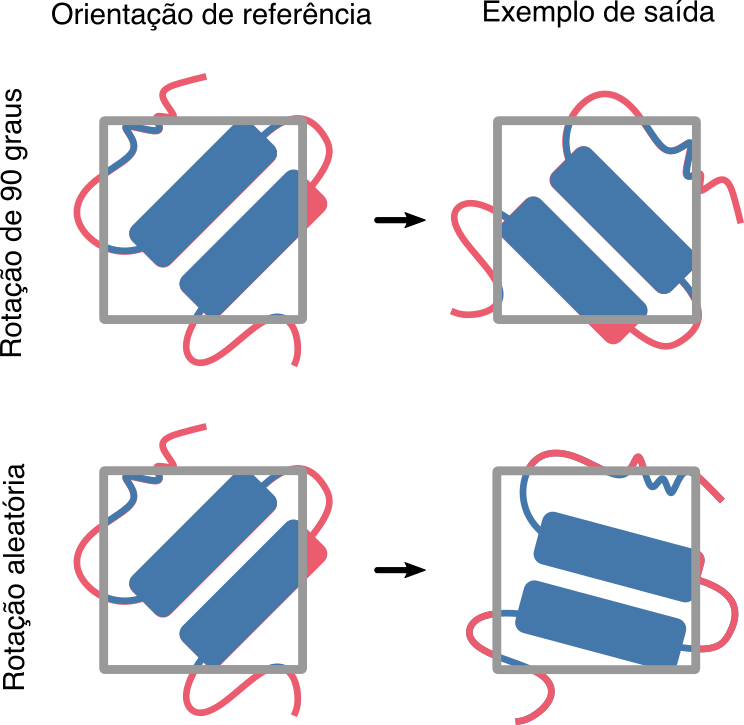
\includegraphics[width=.85\linewidth]{imgs/rotation-types.png}
%             \caption{Different rotations applied to the protein-ligand complex.}
%         \end{figure}
%     \end{columns}
% \end{frame}



\begin{frame}{Literature review: \textit{de novo} design}
    \begin{columns}[c]
        \column{.45\textwidth}
        Three main approaches are employed for the \textit{de novo} design of molecules using generative models:
        \begin{itemize}
            \item Distribution learning
            \item Conditional generation
            \item Objective-guided learning
        \end{itemize}
        % \vspace{1em}
        %Poucos modelos na literatura abordam a geração \textit{de novo} de moléculas como problemas \textit{many}-objetivo ($k>3$ objetivos simultâneos).
        \begin{block}{Current limitations}
            Methodologies that handle $k\geq$4 objectives are still little
            explored in the literature, with few studies considering
            more than three objectives, especially integrating appropriate techniques and generative models~\cite{angelo2023multi}.
        \end{block}

        \column{.45\textwidth}
        \begin{figure}
            \centering
            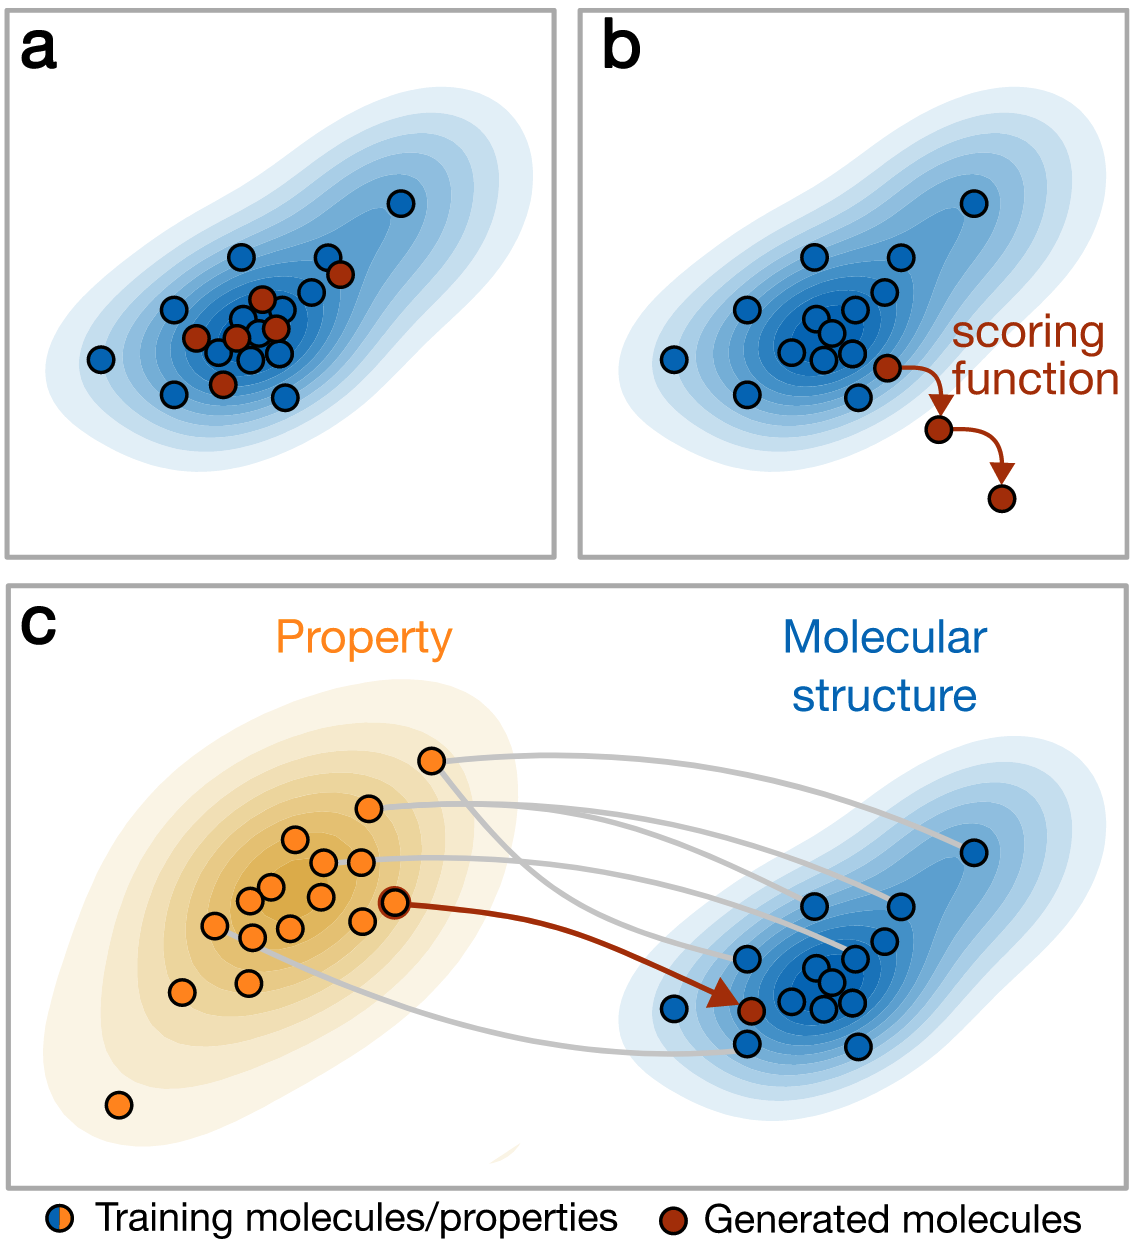
\includegraphics[width=.75\linewidth]{imgs/generation-approaches.png}
            \caption{Generative approaches: (a) distribution learning, (b) objective-guided learning, and (c) conditional generation~\cite{özçelik2025generative}.}
        \end{figure}
    \end{columns}
\end{frame}



% \begin{frame}{Objetivos específicos da tese}
%     \begin{block}{Objetivos específicos}
%         \begin{itemize}
%             \item Avaliar estratégias de aumento de dados por rotação para mitigar a variância rotacional no modelo \alert{DockTDeep}.
%             \item Propor e validar uma nova técnica, chamada dropout molecular, para guiar o modelo no aprendizado de interações (\alert{DockTDeep}).
%             \item Avaliar a capacidade de generalização do modelo \alert{DockTDeep} em diferentes cenários fora de domínio.
%             \item Avaliar o desempenho da plataforma \alert{DockTDesign} na otimização simultânea de até 5~objetivos.
%             \item Investigar o impacto da inclusão de restrições de otimização no desempenho de algoritmos many-objetivo (\alert{DockTDesign}).
%         \end{itemize}
%     \end{block}
% \end{frame}






%%%% DOCKTDESIGN TRANSITION %%%%



% \section{DockTDeep}
% % transtion page 
% \begin{frame}  % transition page
%     \Large{\centerline{\textbf{DockTDeep}}}
% \end{frame}



% \subsection{Methodology}

% \begin{frame}{Dataset: training and validation \hfill {\footnotesize \alert{DockTDeep}}}
%     \begin{columns}[t]
%         \column{.475\textwidth}
%         \begin{block}{PDBbind v.2020}
%             General set: \textbf{19.443} cpxs \\
%             Refined set: \textbf{5.316} cpxs \\
%             Coreset v.2013: \textbf{170} cpxs \\
%             Coreset v.2016: \textbf{261} cpxs \\
%         \end{block}

%         \column{.475\textwidth}
%         \begin{block}{Hyperparameter Search}
%             Using the refined set (random split)
%             \begin{itemize}
%                 \item Training: \textbf{3.599} cpxs
%                 \item Validation: \textbf{904} cpxs
%             \end{itemize}
%         \end{block}

%         % \column{.32\textwidth}

%     \end{columns}

%     \begin{block}{Activity ranges}
%         The validation set data (\textbf{904} cpxs) were divided into activity ranges:
%         \item \textbf{Strong}: $\Delta \text{G}_{\text{bind}} \leq -9.981$ kcal/mol (45 nM).
%         \item \textbf{Moderate}: $-9.981 \; \text{kcal/mol} < \Delta \text{G}_{\text{bind}} \leq  -7.395$ kcal/mol (3.6 $\mu$M).
%         \item \textbf{Weak/inactive}: $\Delta \text{G}_{\text{bind}} > -7.395$ kcal/mol.
%     \end{block}
% \end{frame}


% \begin{frame}{Dataset: external test \hfill {\footnotesize \alert{DockTDeep}}}
%     Performance on test sets was evaluated using the \textit{general set}, in different splits:
%     \begin{itemize}
%         \item Random (15.699 train/3.404 test).
%         \item Temporal (13.317 train/1.786 test).
%         \item \textit{Coreset} v.2013 (18.933 train/170 test).
%         \item \textit{Coreset} v.2016  (18.842 train/261 test).
%               \vspace{1 em}
%         \item Pfam-CV protocol (\textit{general set}):
%               \begin{itemize}
%                   \item Evaluation of out-of-domain generalization.
%                   \item Grouping by structural similarity of the binding site (Pfam database).
%                   \item Repeated cross-validation 30x.
%                   \item Proportion: $\frac{2}{3}$ training and $\frac{1}{3}$ test.
%               \end{itemize}
%     \end{itemize}

% \end{frame}


% \begin{frame}{Molecular representation \hfill {\footnotesize \alert{DockTDeep}}}
%     \begin{columns}[c]
%         \column{.575\textwidth}
%         \begin{itemize}
%             \item Voxel grid 24~{\AA}$^3$ and discretization 1~{\AA}.
%             \item Channels for elements: C, H, O, N, S, and X (others).
%             \item 21 channels: 6 protein, 6 ligand, 6 cpx, and 3 total volume.
%             \item Representations generated with DockTGrid~\cite{dadocktgrid}.
%             \item GitHub: {\color{blue} \href{https://github.com/gmmsb-lncc/docktgrid}{github.com/gmmsb-lncc/docktgrid}}.
%         \end{itemize}

%         \column{.375\textwidth}
%         \begin{figure}
%             \centering
%             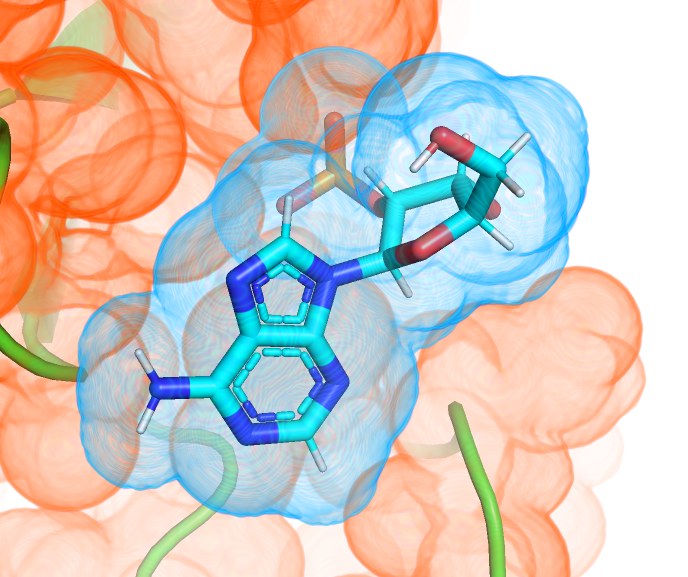
\includegraphics[width=0.9\linewidth]{imgs/cpx-representation.png}
%             \caption{Illustrative example of the voxel representation used.}
%         \end{figure}

%     \end{columns}
% \end{frame}


% \begin{frame}{Neural network architecture \hfill {\footnotesize \alert{DockTDeep}}}
%     \begin{columns}[c]
%         \column{.4\textwidth}
%         \begin{itemize}
%             \item 3D CNN with three convolutional layers.
%             \item One dense layer of 1000 neurons.
%             \item Linear output layer (regression).
%             \item $\sim$2M trainable parameters.
%             \item Learning rate: $8,74\times10^{-4}$
%             \item Training epochs: 1500.
%             \item GitHub: {\color{blue} \href{https://github.com/gmmsb-lncc/docktdeep}{github.com/gmmsb-lncc/docktdeep}} and preprint~\cite{da2025data}.
%         \end{itemize}

%         \column{.55\textwidth}
%         \begin{figure}
%             \centering
%             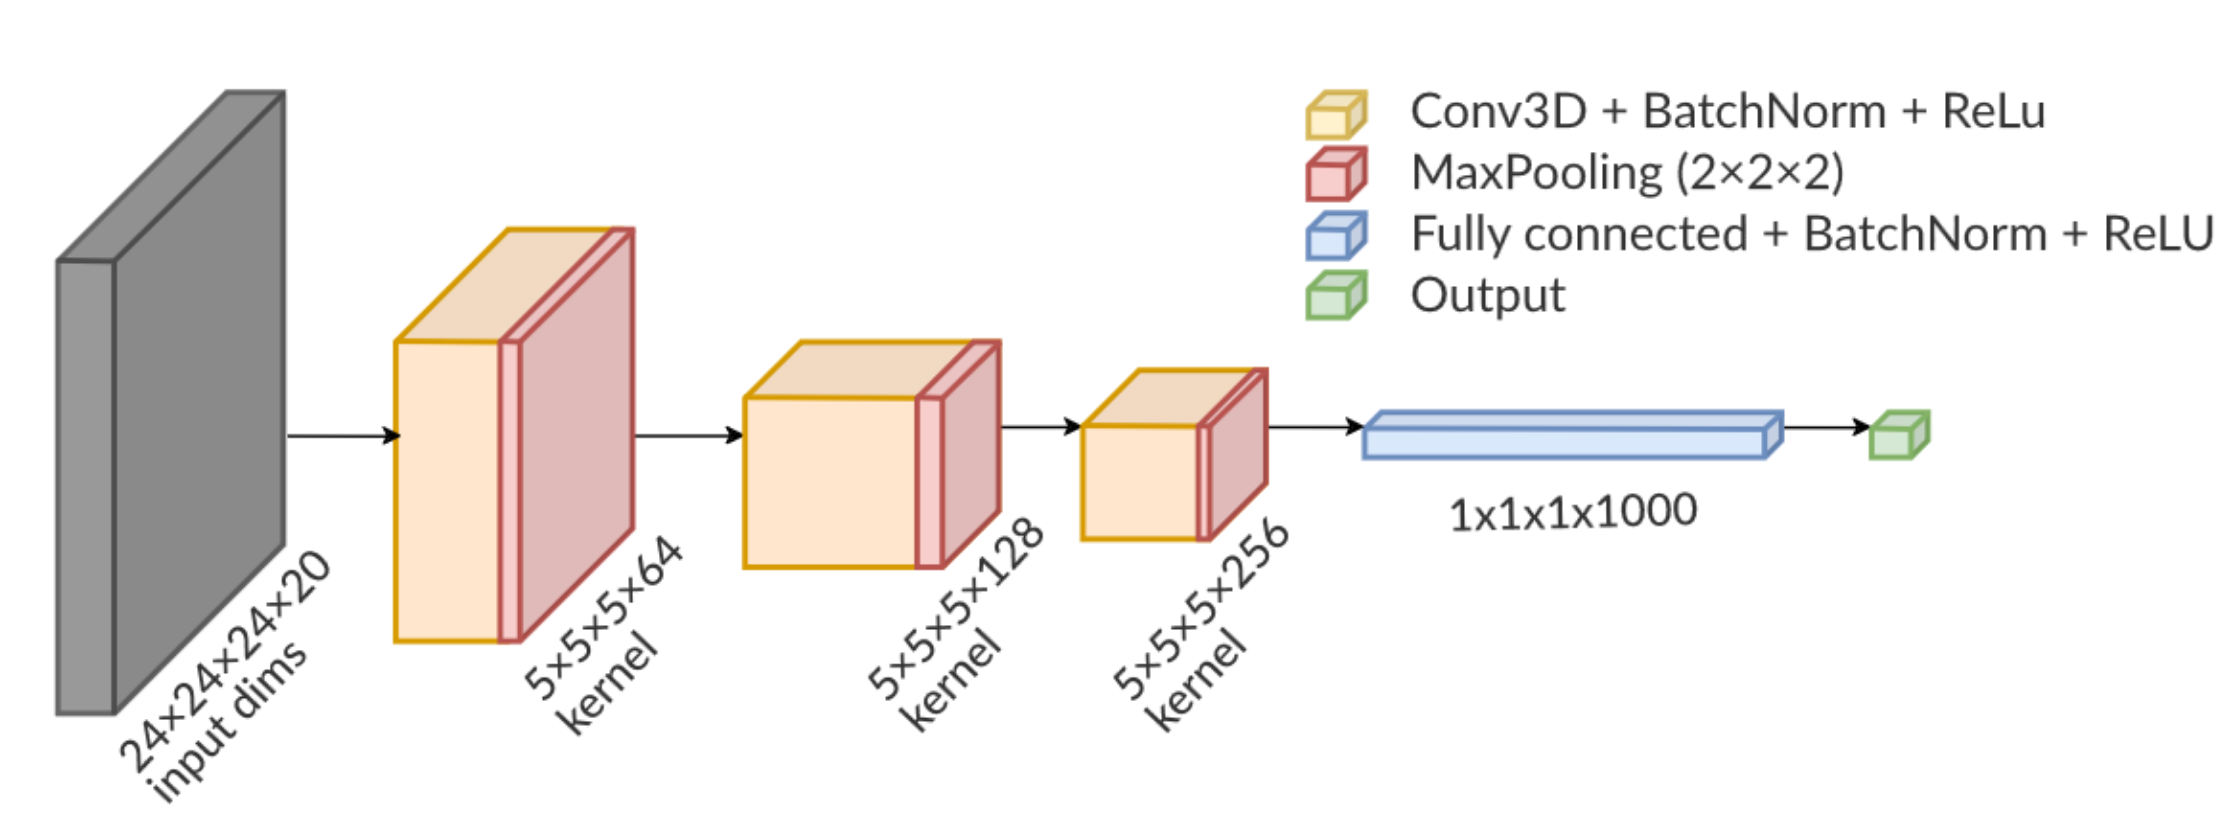
\includegraphics[width=1.\linewidth]{imgs/arquitetura-cnn.png}
%             \caption{CNN network architecture.}
%         \end{figure}
%     \end{columns}
% \end{frame}


% \begin{frame}{Data augmentation strategies \hfill {\footnotesize \alert{DockTDeep}}}
%     \begin{columns}[c]
%         \column{.475\textwidth}
%         Two data augmentation strategies were compared:
%         \begin{itemize}
%             \item 90° rotations;
%             \item random rotations in the complex (applied at each new epoch).
%         \end{itemize}

%         \column{.475\textwidth}
%         \begin{figure}
%             \centering
%             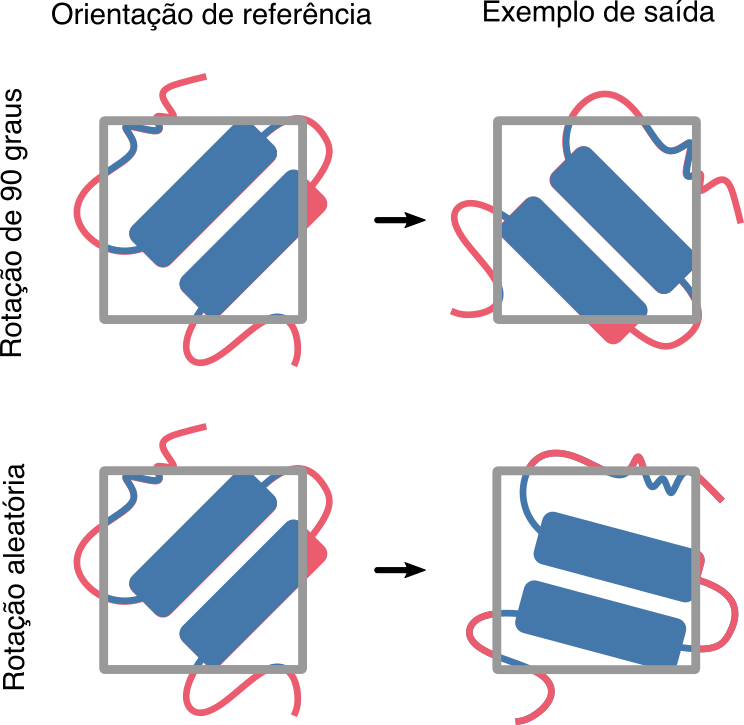
\includegraphics[width=.85\linewidth]{imgs/rotation-types.png}
%             \caption{Different rotations applied to the protein-ligand complex.}
%         \end{figure}

%     \end{columns}
% \end{frame}




% \begin{frame}{Molecular dropout \hfill {\footnotesize \alert{DockTDeep}}}
%     \begin{columns}[c]
%         \column{.475\textwidth}
%         \begin{itemize}
%             \item Regularization technique that avoids overfitting by randomly removing protein \textit{or} ligand during training and setting affinity to zero.
%             \item Each complex has chance $p = 0{,}06$ of undergoing dropout per epoch.
%             \item Seeks to force the model to learn relevant interactions, not depending on a single component.
%         \end{itemize}

%         \column{.475\textwidth}

%         \centering
%         \begin{tikzpicture}[node distance=1.5cm, auto, scale=0.5, every node/.style={transform shape}]
%             % Estilos
%             \tikzset{
%             input/.style = {rectangle, rounded corners, draw=black, fill=red!10, text width=4cm, align=center, inner sep=8pt},
%             decision/.style = {diamond, draw=black, fill=yellow!30, aspect=2, inner sep=1pt, text width=2.5cm, align=center},
%             output/.style = {rectangle, draw=black, fill=green!15, text width=4cm, align=center, inner sep=6pt},
%             arrow/.style = {-{Stealth[length=5pt]}, thick, shorten >=1pt, shorten <=1pt}
%             }

%             % Nós
%             \node [input] (input) {Protein-Ligand Complex};
%             \node [decision, below=of input] (dropout) {Molecular Dropout? \\ (prob. $p$)};
%             \node [decision, below left=1cm and 1.2cm of dropout] (choose) {Protein or Ligand? \\ (50/50)};
%             \node [output, below=of choose] (drop) {Train with \\ only one entity};
%             \node [output, right=2.8cm of drop] (keep) {Train with \\ complete complex};

%             % Setas: uso explícito de anchors nas pontas dos losangos
%             \draw [arrow] (input) -- (dropout.north);

%             % Saída esquerda do losango 'dropout' -> entra pela ponta superior de 'choose'
%             \draw [arrow] (dropout.west) to[out=-150,in=60] node[left, xshift=-1mm] {Yes} (choose.north);

%             % 'choose' para 'drop'
%             \draw [arrow] (choose.south) -- (drop.north);

%             % Saída direita do losango 'dropout' -> caminho em ângulo até 'keep'
%             \draw [arrow] (dropout.east) to[out=-20,in=90] node[midway,right] {No} (keep.north);
%         \end{tikzpicture}



%     \end{columns}
% \end{frame}


% \begin{frame}{Experimentos de atracamento molecular \hfill {\footnotesize \alert{DockTDeep/DockTDesign}}}
%     \begin{block}{Configuração dos experimentos}
%         \begin{itemize}
%             \item Programa: \textbf{DockThor}, campo de força \textbf{MMFF94S}.
%             \item 24 rodadas\footnote{No caso do \alert{DockTDesign}, apenas 1 rodada foi utilizada.}, 750 indivíduos, 1M avaliações por rodada.
%             \item Poses ranqueados pela \textit{E$_{total}$}.
%             \item \textbf{``Pose incorreta''}: maior RMSD entre as 10 melhores.
%         \end{itemize}
%     \end{block}
% \end{frame}



% \begin{frame}{Fingerprints de interação receptor-ligante \hfill {\footnotesize \alert{DockTDeep}}}
%     \begin{columns}[t]
%         \column{.475\textwidth}
%         \begin{block}{Geração dos IFPs}
%             \begin{itemize}
%                 \item Método: \textbf{PLEC} (4,5~{\AA} de corte).
%                 \item Profundidade: 4 (prot.) / 2 (lig.).
%                 \item Vetor: \textbf{4096 bits}.
%                 \item Ferramenta: \textbf{ODDT v0.7}.
%             \end{itemize}
%         \end{block}

%         \column{.475\textwidth}
%         \begin{block}{Similaridade Dice}
%             \begin{itemize}
%                 \item Métrica para vetores binários:
%                       \[
%                           \text{Dice}(a,b) = \frac{2 \sum \min(a_i,b_i)}{\sum a_i + \sum b_i}
%                       \]
%                 \item Comparação iterativa entre conjuntos através da \textbf{similaridade máxima}.
%             \end{itemize}
%         \end{block}
%     \end{columns}
% \end{frame}



% \begin{frame}{Algoritmo $k$-NN \hfill {\footnotesize \alert{DockTDeep}}}
%     \begin{columns}[t]
%         \column{.475\textwidth}
%         \begin{block}{Predição de afinidade}
%             \begin{itemize}
%                 \item Modelo base: \textbf{k-NN} por similaridade de ligantes.
%                 \item Predição: média das afinidades dos $k$ vizinhos mais próximos:
%                       \[
%                           \hat{y} = \frac{1}{k} \sum_{i=1}^{k} y_i
%                       \]
%                 \item Valor usado: \textbf{$k = 5$}.
%             \end{itemize}
%         \end{block}

%         \column{.475\textwidth}
%         \begin{block}{Similaridade Tanimoto}
%             \begin{itemize}
%                 \item Fingerprints: \textbf{Morgan (ECFP)}, raio 2 (\textbf{RDKit}).
%                       \[
%                           \text{TS}(A,B) = \frac{|A \cap B|}{|A \cup B|}
%                       \]
%                 \item $|A \cap B|$: bits 1 em comum.
%                 \item $|A \cup B|$: bits 1 em qualquer fingerprint.
%             \end{itemize}
%         \end{block}
%     \end{columns}
% \end{frame}

% \subsection{Results}

% % transition frame (Resultados)
% \begin{frame}  % transition page
%     \Large{\centerline{\textbf{Results}}}
% \end{frame}

% \begin{frame}{Results: rotational variance \hfill {\footnotesize \alert{DockTDeep}}}
%     \begin{columns}[c]
%         \column{.475\textwidth}

%         \begin{figure}
%             \centering
%             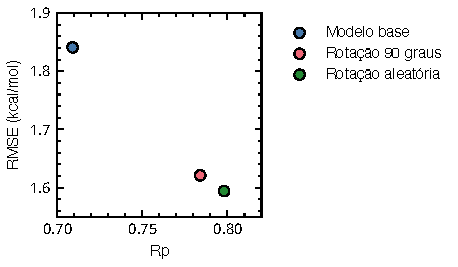
\includegraphics[width=1\linewidth]{imgs/results/rotation-performance.pdf}
%             \caption{Comparison of predictive performance using RMSE (lower is better) and Rp (higher is better) metrics for each strategy.}
%         \end{figure}

%         \column{.475\textwidth}

%         \begin{figure}
%             \centering
%             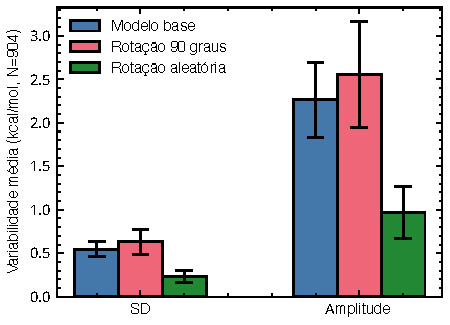
\includegraphics[width=1\linewidth]{imgs/results/mean-variances.pdf}
%             \caption{Mean standard deviation (SD) and range of predictions (kcal/mol) for the validation set (N=904).}
%         \end{figure}

%         % \begin{figure}
%         %     \centering
%         %     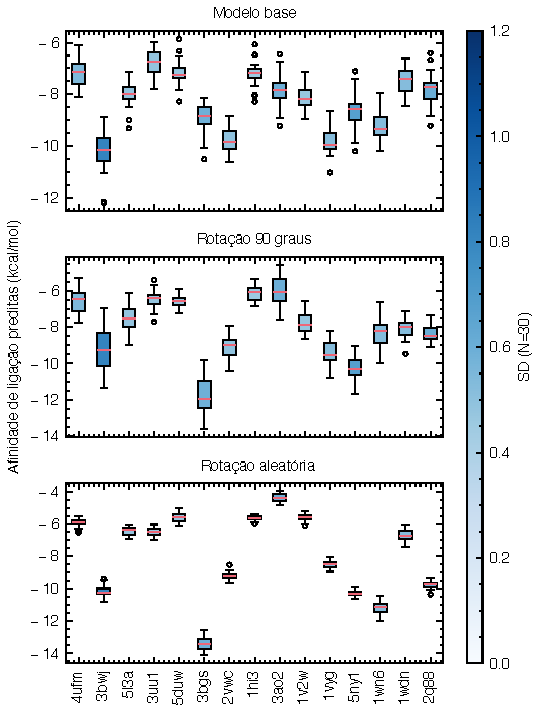
\includegraphics[width=0.7\linewidth]{imgs/results/rotation-variance.pdf}
%         %     \caption{Distribution of affinity values.}
%         % \end{figure}

%     \end{columns}
% \end{frame}



% \begin{frame}{Results: protein/ligand bias \hfill {\footnotesize \alert{DockTDeep}}}
%     \begin{figure}
%         \centering
%         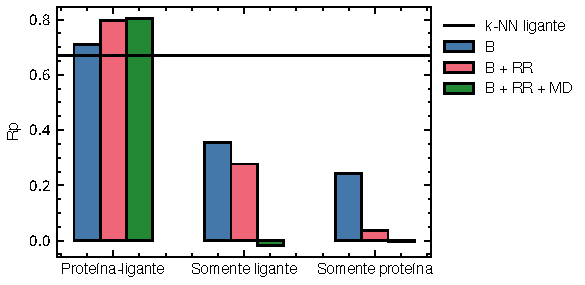
\includegraphics[width=0.7\linewidth]{imgs/results/ligand-bias.pdf}
%         \caption{Comparison of Rp values between three models: base model (B), using random rotation (B + RR), and using random rotation and molecular dropout (B + RR + MD), in addition to the k-NN model based only on the ligand. Evaluation was performed in three distinct scenarios: complete protein-ligand complex, ligand only, and protein only; keeping affinity labels unchanged.}
%     \end{figure}
% \end{frame}


% \begin{frame}{Results: protein/ligand bias \hfill {\footnotesize \alert{DockTDeep}}}
%     \begin{columns}[c]
%         \column{.495\textwidth}
%         \begin{figure}
%             \centering
%             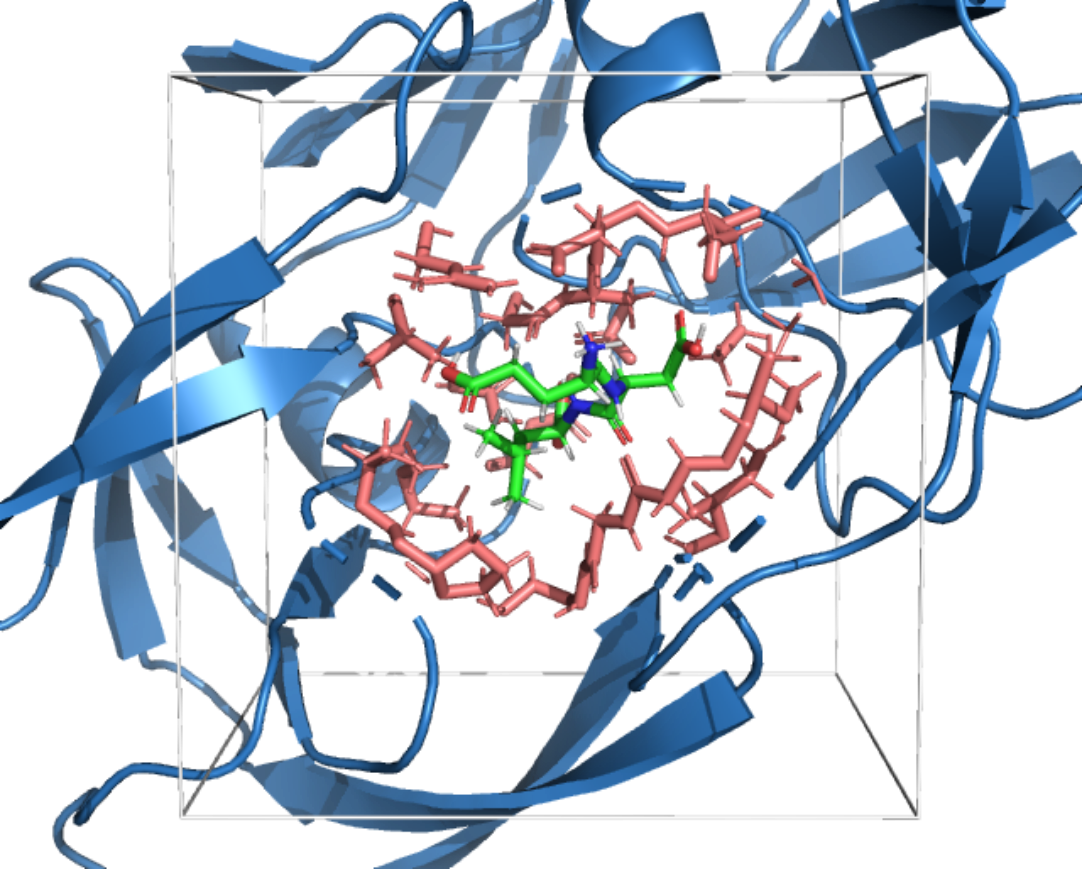
\includegraphics[width=.8\textwidth]{imgs/results/masking.png}
%             \caption{Visualization of removed protein atoms (highlighted in red), which are up to 5~\AA{} from the ligand.}
%         \end{figure}

%         \column{.495\textwidth}
%         \begin{figure}
%             \centering
%             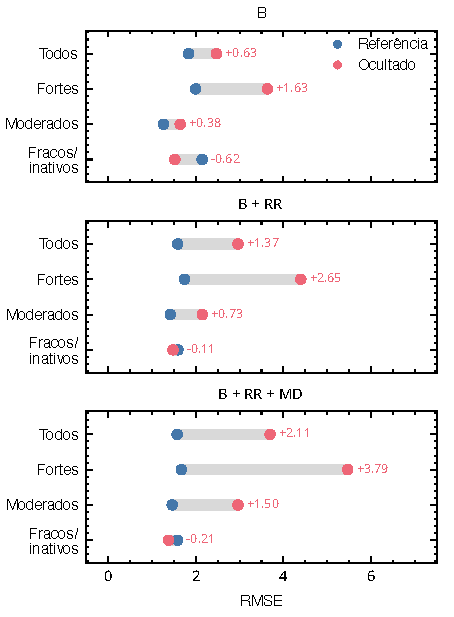
\includegraphics[width=.65\textwidth]{imgs/results/masking-rmse.pdf}
%             \caption{RMSE before (blue) and after atom removal (red).}
%         \end{figure}
%     \end{columns}
% \end{frame}


% \begin{frame}{Results: learning of interactions \hfill {\footnotesize \alert{DockTDeep}}}
%     \begin{figure}
%         \centering
%         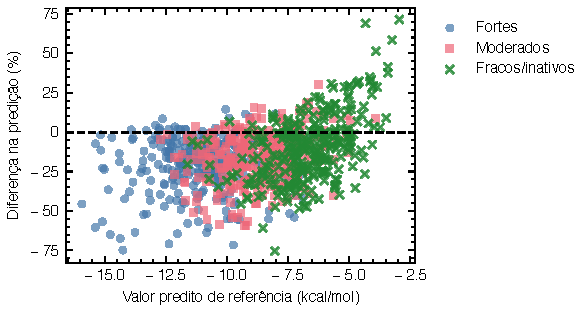
\includegraphics[width=0.6\textwidth]{imgs/results/pose-sensitivity.pdf}
%         \caption{Scatter plot comparing affinity predictions for crystallographic structures (reference) with the percentage variation in predictions for the worst poses obtained in the redocking experiment.}
%     \end{figure}
% \end{frame}


% \begin{frame}{Results: activity ranges \hfill {\footnotesize \alert{DockTDeep}}}
%     \begin{columns}[c]
%         \column{.475\textwidth}
%         \begin{figure}
%             \centering
%             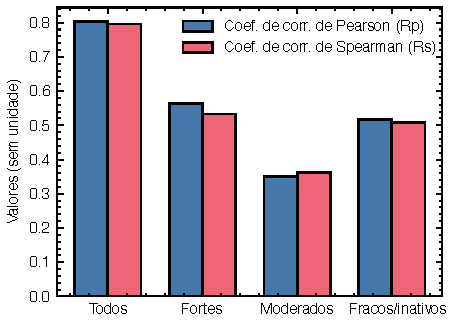
\includegraphics[width=0.9\textwidth]{imgs/results/correlations-in-range-2.pdf}
%             \caption{Comparison of Rp and Rs values for the entire validation set and affinity ranges.}
%         \end{figure}

%         \column{.475\textwidth}
%         \begin{figure}
%             \centering
%             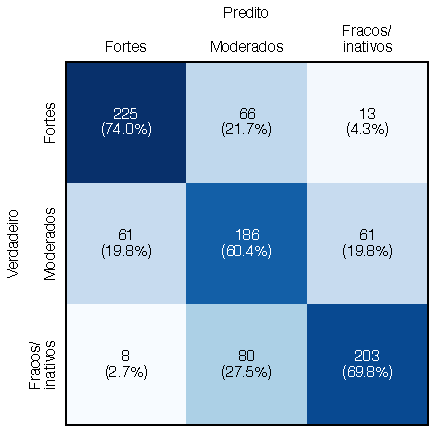
\includegraphics[width=.85\textwidth]{imgs/results/confusion-matrix.pdf}
%             \caption{Confusion matrix for the three affinity classes: strong, moderate, and weak/inactive.}
%         \end{figure}
%     \end{columns}
% \end{frame}


% \begin{frame}{Resultados: falsos negativos \hfill {\footnotesize \alert{DockTDeep}}}
%     \small
%     \begin{center}
%         \begin{tabular}{lccp{7cm}}
%             \toprule
%             \textbf{PDB ID} & \textbf{Pred.} & \textbf{Exp.} & \textbf{Possível razão da classificação incorreta}                                                 \\
%             \midrule
%             2CCB            & -7.24          & -10.15        & Cristal possui múltiplos ligantes na mesma região; no PDBbind apenas uma ocorrência está presente. \\[0.3em]
%             3DSZ            & -7.13          & -10.59        & Ligante coordena o metal Y (ítrio), ausente no PDBbind.                                            \\[0.3em]
%             2YLC$^{\star}$  & -6.55          & -10.75        & Ligante é um homo-hexâmero; no PDBbind apenas uma unidade está presente.                           \\[0.3em]
%             4O2C            & -7.05          & -10.90        & Afinidade erroneamente reportada no PDBbind.                                                       \\[0.3em]
%             5D21            & -6.90          & -11.34        & Ligante é um polímero; no PDBbind apenas uma subunidade está presente.                             \\
%             \bottomrule
%         \end{tabular}
%     \end{center}

%     \vspace{0.5em}
%     \footnotesize
%     \textbf{Nota:} Valores de $\Delta$G em kcal/mol. Pred. = Predito, Exp. = Experimental.
% \end{frame}


% \begin{frame}{Resultados: falsos positivos \hfill {\footnotesize \alert{DockTDeep}}}
%     \small
%     \begin{center}
%         \begin{tabular}{lccp{7cm}}
%             \toprule
%             \textbf{PDB ID} & \textbf{Pred.} & \textbf{Exp.} & \textbf{Possível razão da classificação incorreta}      \\
%             \midrule
%             4XOE            & -11.41         & -6.82         & Afinidade experimental devido a uma alosteria dinâmica. \\[0.3em]
%             3N9S            & -10.34         & -7.17         & Afinidade erroneamente reportada no PDBbind.            \\
%             \bottomrule
%         \end{tabular}
%     \end{center}

%     \vspace{0.5em}
%     \footnotesize
%     \textbf{Nota:} Valores de $\Delta$G em kcal/mol. Pred. = Predito, Exp. = Experimental.
% \end{frame}




% \begin{frame}{Resultados: inclusão de dados ruidosos \hfill {\footnotesize \alert{DockTDeep}}}
%     \begin{figure}
%         \centering
%         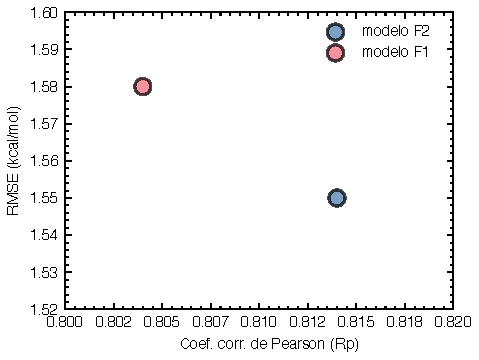
\includegraphics[width=.45\textwidth]{imgs/results/data-quality.pdf}
%         \caption{Comparação do desempenho preditivo entre modelos treinados com diferentes conjuntos de dados (F1=refined, F2=general).  Ambos os modelos foram avaliados no mesmo conjunto de validação (N=904).}
%     \end{figure}

% \end{frame}


% \begin{frame}{Results: evaluation on external sets \hfill {\footnotesize \alert{DockTDeep}}}
%     \begin{columns}[c]
%         \column{.495\textwidth}
%         \begin{figure}
%             \centering
%             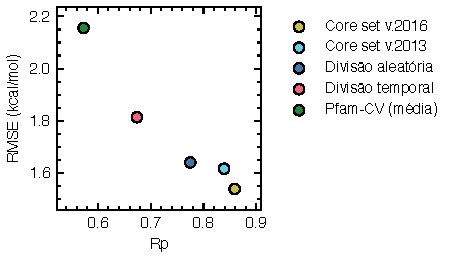
\includegraphics[width=1\textwidth]{imgs/results/fig5a_external_performance.pdf}
%             \caption{Comparison of RMSE (lower is better) and Rp (higher is better) values in all evaluated test sets.}
%         \end{figure}

%         \column{.495\textwidth}
%         \begin{figure}[ht!]
%             \centering
%             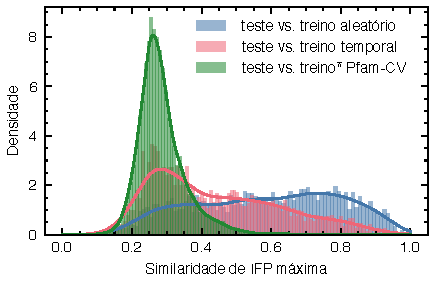
\includegraphics[width=1\textwidth]{imgs/results/ifp-similarity.pdf}
%             \caption{Density plot of maximum IFP similarity between sets.}
%         \end{figure}

%     \end{columns}
% \end{frame}



% \begin{frame}{Results: PDBbind coresets & Pfam-CV \hfill {\footnotesize \alert{DockTDeep}}}
%     \begin{columns}[c]
%         \column{.475\textwidth}
%         \begin{figure}
%             \centering
%             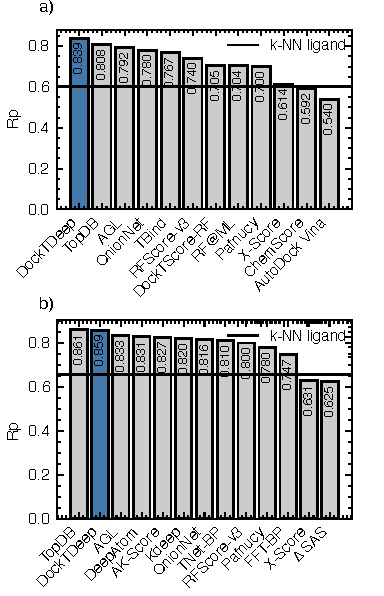
\includegraphics[width=.6\textwidth]{imgs/results/fig5b_coreset16_comparison_up.pdf}
%             \caption{Rp in PDBbind v. (a) 2013 and (b) 2016.}
%         \end{figure}

%         \column{.475\textwidth}
%         \begin{figure}
%             \centering
%             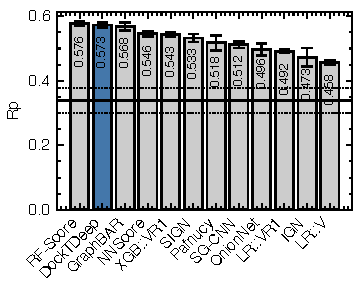
\includegraphics[width=.7\textwidth]{imgs/results/fig5c_pfam_external_performance.pdf}
%             \caption{Rp in the Pfam-CV split scheme.}
%         \end{figure}
%     \end{columns}

% \end{frame}



% \begin{frame}{Conclusions \hfill {\footnotesize \alert{DockTDeep}}}

%     \begin{itemize}
%         \item \textbf{DockTDeep}: simple 3D CNN model, trained in a systematic and grounded manner, shows robust generalization and is competitive with the state of the art.

%         \item Random rotation surpasses 90° rotation as a data augmentation technique, improving stability and performance.

%         \item Molecular dropout reduces protein/ligand bias, favoring learning of significant interactions.

%         \item Model is more robust in \textbf{categorization} tasks (strong/moderate/weak) than in fine ranking.

%         \item Performance drops in rigorous scenarios (Pfam-CV), highlighting limitations imposed by the diversity of training and test data.
%     \end{itemize}

% \end{frame}



% %%%% DOCKTDESIGN TRANSITION %%%%



% \section{DockTDesign}
% % transtion page 
% \begin{frame}  % transition page
%     \Large{\centerline{\textbf{DockTDesign}}}
% \end{frame}



\subsection{Methodology}

\begin{frame}{Generative chemistry model \hfill {\footnotesize \alert{DockTDesign}}}
    \begin{columns}[t]
        \column{.475\textwidth}
        \begin{itemize}
            \item \textbf{HierVAE} model based on graphs for generation of molecules with \textbf{100\% validity}~\cite{jin2020hierarchical}.
            \item Uses \textbf{structural motifs} as building blocks, extracted from recurring patterns in ChEMBL.
            \item Representation in \textbf{3 levels}: motifs, bonds between motifs, and atomic graph.
            \item Regular latent space ($z \in \mathbb{R}^{32}$).
            \item Pre-trained on \textbf{1.8M molecules} from ChEMBL.
        \end{itemize}

        \column{.475\textwidth}
        \begin{figure}
            \centering
            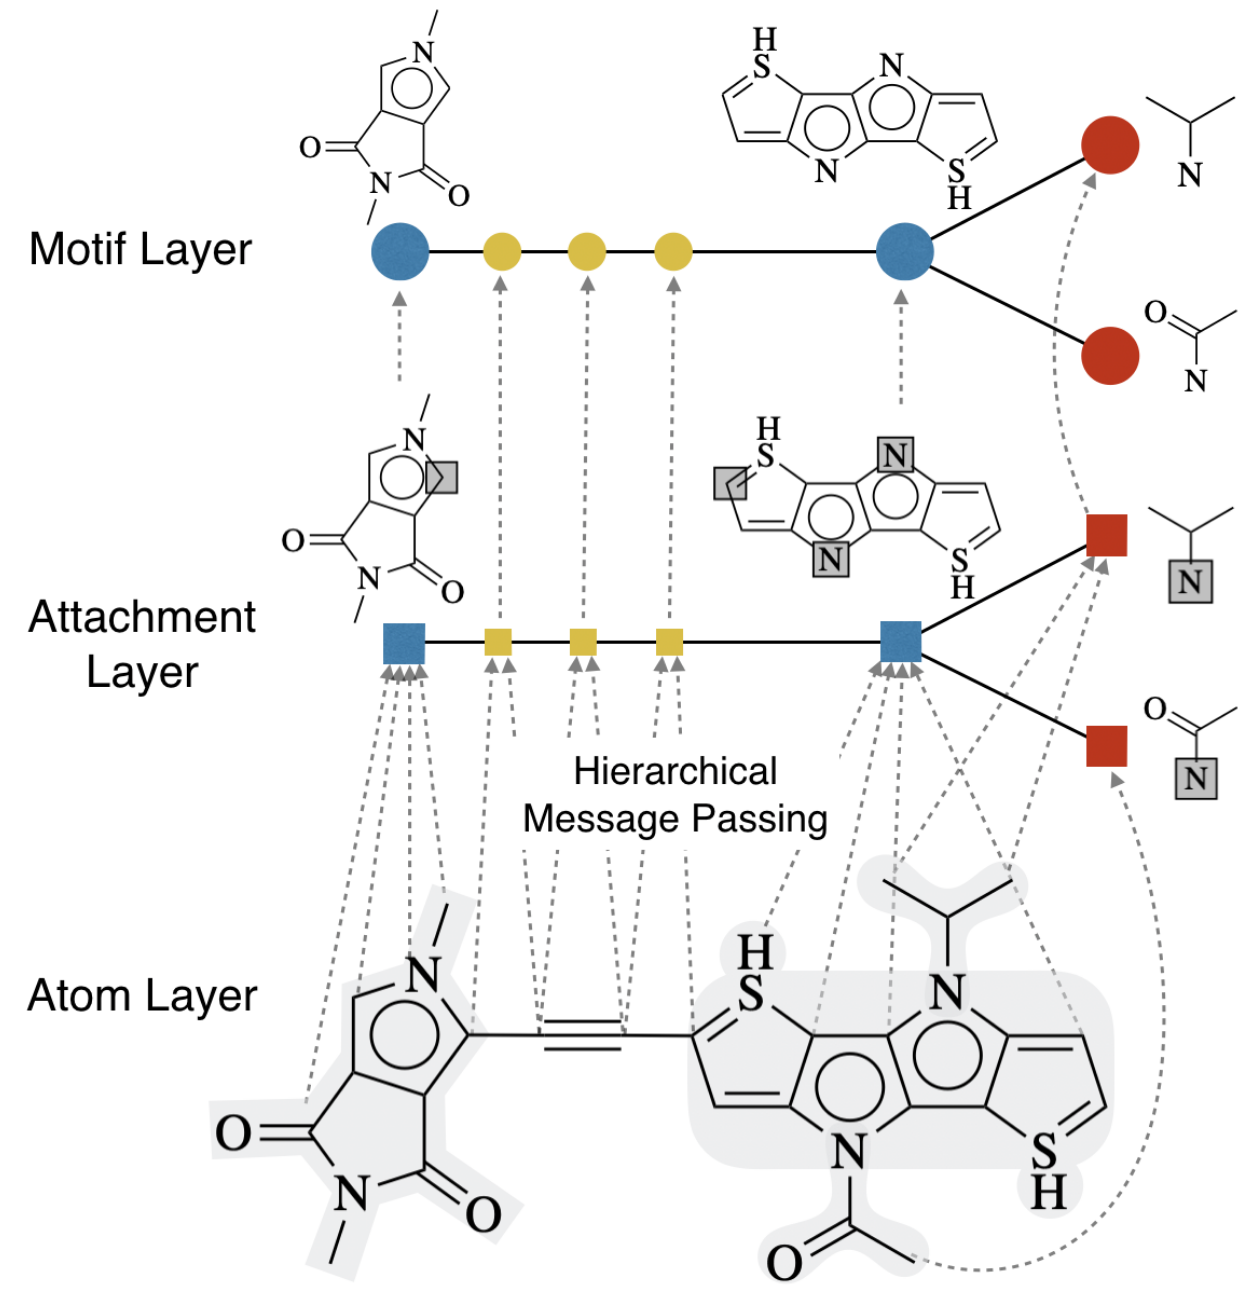
\includegraphics[width=0.785\linewidth]{imgs/hiervae-encoder.png}
            \caption{Hierarchical encoder of the HierVAE model~\cite{jin2020hierarchical}.}
        \end{figure}
    \end{columns}
\end{frame}


\begin{frame}{Multi-objective evolutionary algorithms \hfill {\footnotesize \alert{DockTDesign}}}
    \begin{columns}[t]
        \column{.475\textwidth}
        \textbf{Compared algorithms:}
        \begin{itemize}
            \item NSGA-II (multi-objective).
            \item NSGA-III (\textit{many}-objective).
            \item Single-objective GA with aggregation.
        \end{itemize}

        \vspace{0.75em}
        \textbf{General execution:}
        \begin{itemize}
            \item 100 generations.
            \item Population: 800 individuals.
            \item 11 independent runs per configuration (only 1 run when using molecular docking).
        \end{itemize}

        \column{.475\textwidth}
        \textbf{Genetic operators:}
        \begin{itemize}
            \item 2-point crossover, $p_c = 0{,}9$.
            \item Gaussian mutation, $p_m = 0{,}1$, $\sigma = 0{,}01$.
            \item Selection: Binary tournament.
        \end{itemize}

        \vspace{0.75em}
        \textbf{Specific configurations:}
        \begin{itemize}
            \item NSGA-III: reference directions via Das-Dennis method (num. equal to population size).
            \item Single-objective GA: 5 weight combinations $(0.6, 0.1, 0.1, 0.1, 0.1)$ to $(0.1, 0.1, 0.1, 0.1, 0.6)$.
        \end{itemize}
    \end{columns}
\end{frame}


\begin{frame}{Proposed generative platform \hfill {\footnotesize \alert{DockTDesign}}}
    \begin{figure}
        \centering
        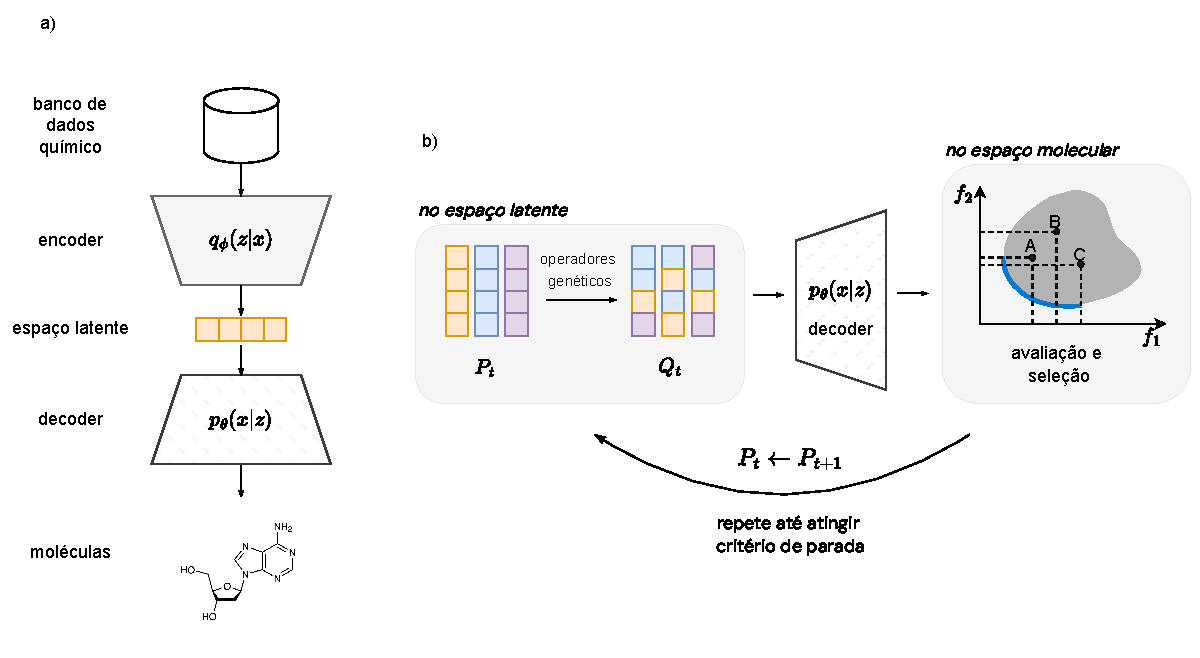
\includegraphics[width=.825\linewidth]{imgs/generative-framework.pdf}
        \vspace{-0.5em}
        \caption{DockTDesign generative platform.}
    \end{figure}
\end{frame}




\begin{frame}{Pharmacological targets \hfill {\footnotesize \alert{DockTDesign}}}
    \begin{columns}[c]
        \column{.495\textwidth}
        A \textbf{target} and an \textbf{anti-target} (\textit{off-target}) were selected as a case study for generating selective inhibitors:
        \begin{itemize}
            \item LpxC\footnote{UDP-3-O-acyl-N-acetylglucosamine deacetylase} (\textbf{target} antimicrobial involved in LPS synthesis).
            \item MMP-9\footnote{matrix metalloproteinase 9} (\textbf{anti-target} human important for extracellular matrix degradation).
        \end{itemize}
        \vspace{1em}
        The choice of targets was made based on the identification of a potent LpxC inhibitor that also inhibits MMP-9 (BDBM50478376).
        \vspace{1em}

        \column{.495\textwidth}
        \begin{figure}
            \centering
            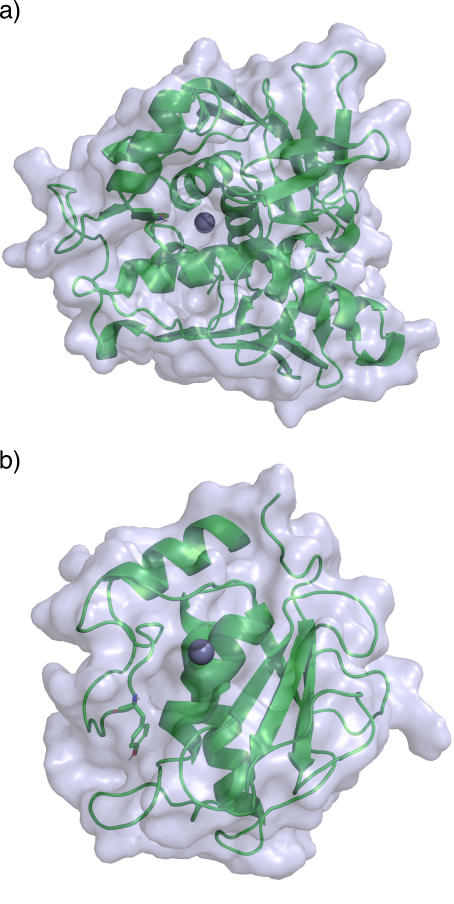
\includegraphics[width=.45\linewidth]{imgs/lpxc_mmp9_receptors.png}
            \caption{Receptors (a) LpxC and (b) MMP-9.}
        \end{figure}
    \end{columns}



    % Structures:
    % \begin{itemize}
    %     \item LpxC: PDB \texttt{3P3G} (comparative model for \textit{K. pneumoniae}).
    %     \item MMP-9: PDB \texttt{4WZV}.
    % \end{itemize}

\end{frame}

\begin{frame}{Optimization objectives and constraints \hfill {\footnotesize \alert{DockTDesign}}}
    \vspace{-1em}
    \begin{columns}[t]
        % Left column
        \column{.49\textwidth}

        \begin{block}{\textit{Drug-likeness} (QED)}
            Maximize similarity to the profile of approved drugs.
            \[
                f_{\text{QED}}(m) = 1 - \text{QED}(m)
            \]
            QED values $\in$ [0,1].
        \end{block}

        % \vspace{1em}

        \begin{block}{Synthetic Accessibility (SA)}
            Penalize molecules that are difficult to synthesize.
            \[
                f_{\text{SA}}(m) = (\text{SA}(m) - 1)^2
            \]
            SA(m) $\in$ [1,10].
        \end{block}

        % Right column
        \column{.49\textwidth}

        \begin{block}{Molecular Weight (MW)}
            Optimize desired target value.
            \[
                f_{\text{MW}}(m, v) = (\text{MW}(m) - v)^2
            \]
            MW$(m)$: mass in Da; $v$: target value.
        \end{block}

        \vspace{1.2em}

        \begin{block}{Molecular Complexity (Cx)}
            Minimize structural complexity.
            \[
                f_{\text{Cx}}(m) = \text{Cx}(m)^2
            \]
            $Cx \in [0, \infty]$.
        \end{block}

    \end{columns}
\end{frame}


\begin{frame}{Objectives: Tanimoto similarity \hfill {\footnotesize \alert{DockTDesign}}}
    \begin{columns}[c]
        \column{.375\textwidth}
        \alert{1. Tanimoto similarity} against molecule BDBM50074960 (K$_i=0.053$ nM LpxC):
        \begin{equation*}
            f_{{\text{sim}}}(m, m_{\text{ref}}) \stackrel{\mathrm{def}}{=} 1 - \text{TS}(m, m_{\text{ref}}).
        \end{equation*}

        \vspace{1em}

        \alert{2. Tanimoto dissimilarity} against molecule BDBM50478376 (K$_i=0.069$ nM LpxC; IC$_{50}=97$ nM MMP-9):

        \begin{equation*}
            f_{{\text{dissim}}}(m, m'_{\text{ref}}) \stackrel{\mathrm{def}}{=} \text{TS}(m, m'_{\text{ref}}),
        \end{equation*}

        \column{.575\textwidth}
        \begin{figure}
            \centering
            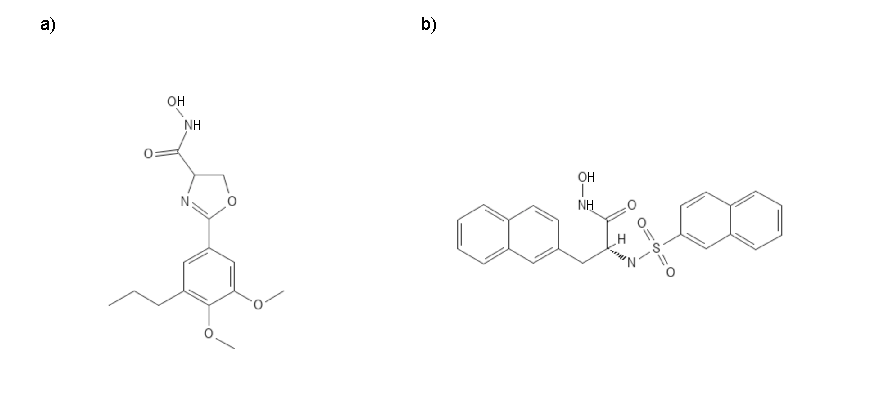
\includegraphics[width=1.2\linewidth]{imgs/ts-compounds.pdf}
            \caption{Compound (a) BDBM50074960 and (b) BDBM50478376}
        \end{figure}
    \end{columns}
\end{frame}


\begin{frame}{Objectives: molecular docking \hfill {\footnotesize \alert{DockTDesign}}}
    Integration \alert{DockTDesign} (generative), \alert{DockThor} (pose) and \alert{DockTDeep} (binding affinity):
    \begin{itemize}
        % \item Função objetivo para otimização da afinidade de ligação:
        \[
            f_{\text{docking}}(m, p, v) = (v - \hat{y}(m, p))^2,
        \]
        where $m$: molecule, $p$: protein target, $v$: target value, $\hat{y}$: affinity prediction (\alert{DockTDeep}).

        \item \textbf{Target}: $v = -25$ kcal/mol (maximize activity).
        \item \textbf{Anti-target}: $v = 0$ kcal/mol (minimize activity).
    \end{itemize}


\end{frame}






\subsection{Results}
% transition frame (Resultados)
\begin{frame}  % transition page
    \Large{\centerline{\textbf{Resultados}}}
\end{frame}

\begin{frame}{Results: Tanimoto similarity \hfill {\footnotesize \alert{DockTDesign}}}
    \begin{block}{Experimental design}
        \textbf{Algorithms:} Single-objective GA, NSGA-II and NSGA-III.

        \vspace{0.5em}

        \textbf{Objectives}:
        \begin{itemize}
            \item[1.] maximize QED;
            \item[2.] minimize SA;
            \item[3.] minimize complexity;
            \item[4.] maximize similarity against molecule BDBM50074960 (active LpxC);
            \item[5.] minimize similarity against molecule BDBM50478376 (active LpxC, active MMP-9).
        \end{itemize}
    \end{block}
    \small Work resulted in a publication in an international conference~\cite{da2024generative}.
\end{frame}


% \begin{frame}{Resultados: similaridade de Tanimoto \hfill {\footnotesize \alert{DockTDesign}}}
%     \begin{figure}[ht!]
%         \centering
%         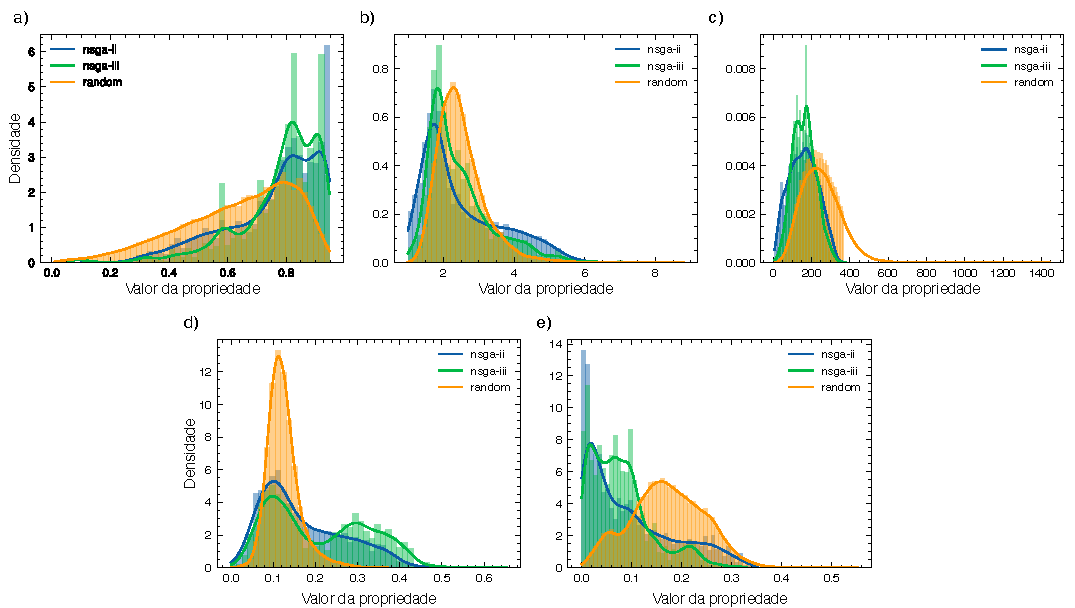
\includegraphics[width=.75\textwidth]{imgs/results/dists.pdf}
%         \caption{Distribuições das propriedades moleculares das soluções não dominadas. Propriedades moleculares: (a) QED, (b) SA, (c) complexidade molecular, (d) similaridade de Tanimoto e (e) dissimilaridade.}
%     \end{figure}
% \end{frame}


\begin{frame}{Results: Tanimoto similarity \hfill {\footnotesize \alert{DockTDesign}}}
    \begin{columns}[c]
        \column{.395\textwidth}
        \begin{table}[ht!]
            \centering
            \footnotesize
            \caption{Multi-objective performance indicators.}
            \begin{tabular}{@{}lll@{}}
                \toprule
                Algo.          & HV\footnotemark[1] & IGD\footnotemark[2] \\ \midrule
                Single-obj. GA & 0.783              & 0.073               \\
                NSGA-II        & 0.805              & 0.040               \\
                NSGA-III       & \textbf{0.880}     & \textbf{0.031}      \\ \bottomrule
            \end{tabular}
            \footnotetext[1]{Hypervolume.}
            \footnotetext[2]{Inverted generational distance.}
        \end{table}

        \column{.595\textwidth}
        \begin{table}[ht!]
            \centering
            \footnotesize
            \caption{Generative chemistry metrics.}
            \begin{tabular}{@{}lllll@{}}
                \toprule
                Algo.    & Valid.\footnotemark[3] & Unic.\footnotemark[4] & DivInt\footnotemark[5] & Nov.\footnotemark[6] \\ \midrule
                NSGA-II  & \textbf{1.00±0.0}      & \textbf{1.00±0.0}     & \textbf{0.70±0.01}     & 0.87±0.01            \\
                NSGA-III & \textbf{1.00±0.0}      & 0.75±0.03             & 0.65±0.01              & \textbf{0.93±0.01}   \\ \bottomrule
            \end{tabular}
            \footnotetext[3]{Validity.}
            \footnotetext[4]{Uniqueness@FP.}
            \footnotetext[5]{Internal diversity.}
            \footnotetext[6]{Novelty.}
        \end{table}
    \end{columns}

\end{frame}


\begin{frame}{Results: Tanimoto similarity \hfill {\footnotesize \alert{DockTDesign}}}
    \begin{columns}[c]
        \column{.495\textwidth}
        \begin{figure}[ht!]
            \centering
            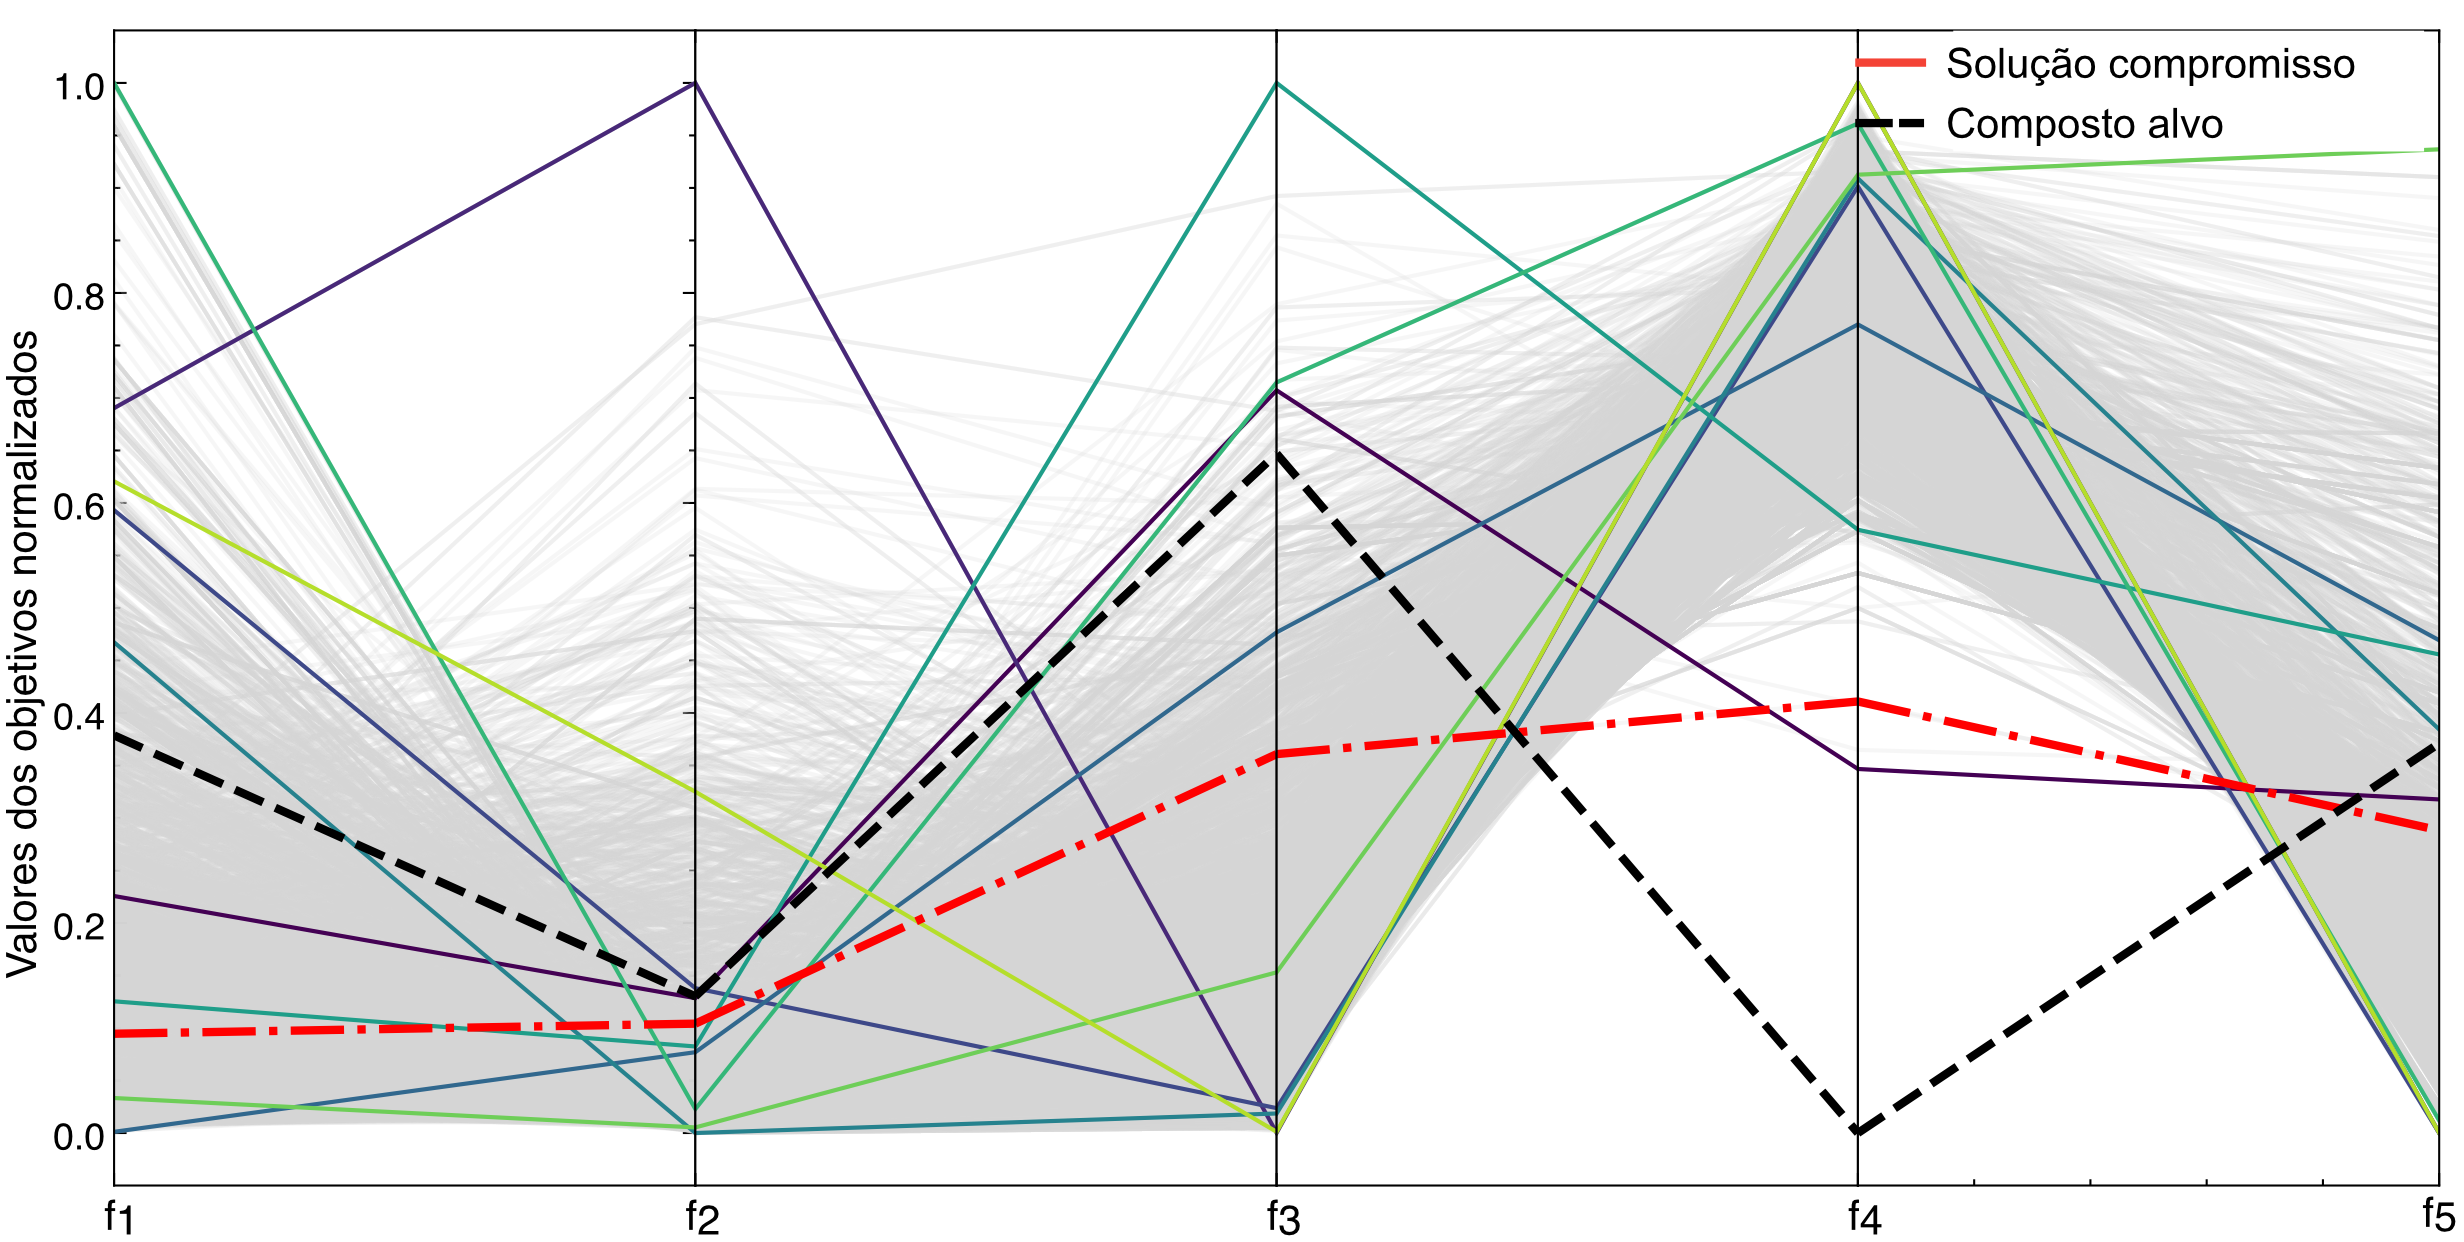
\includegraphics[width=1\textwidth]{imgs/results/parallel-coords.png}
            \caption{Non-dominated solutions generated by the NSGA-III algorithm. Order: $f_{\text{QED}},  f_{\text{SA}}, f_{\text{Cx}},  f_{\text{sim}}, f_{\text{dissim}}$.}
        \end{figure}

        \column{.495\textwidth}
        \begin{figure}[ht!]
            \centering
            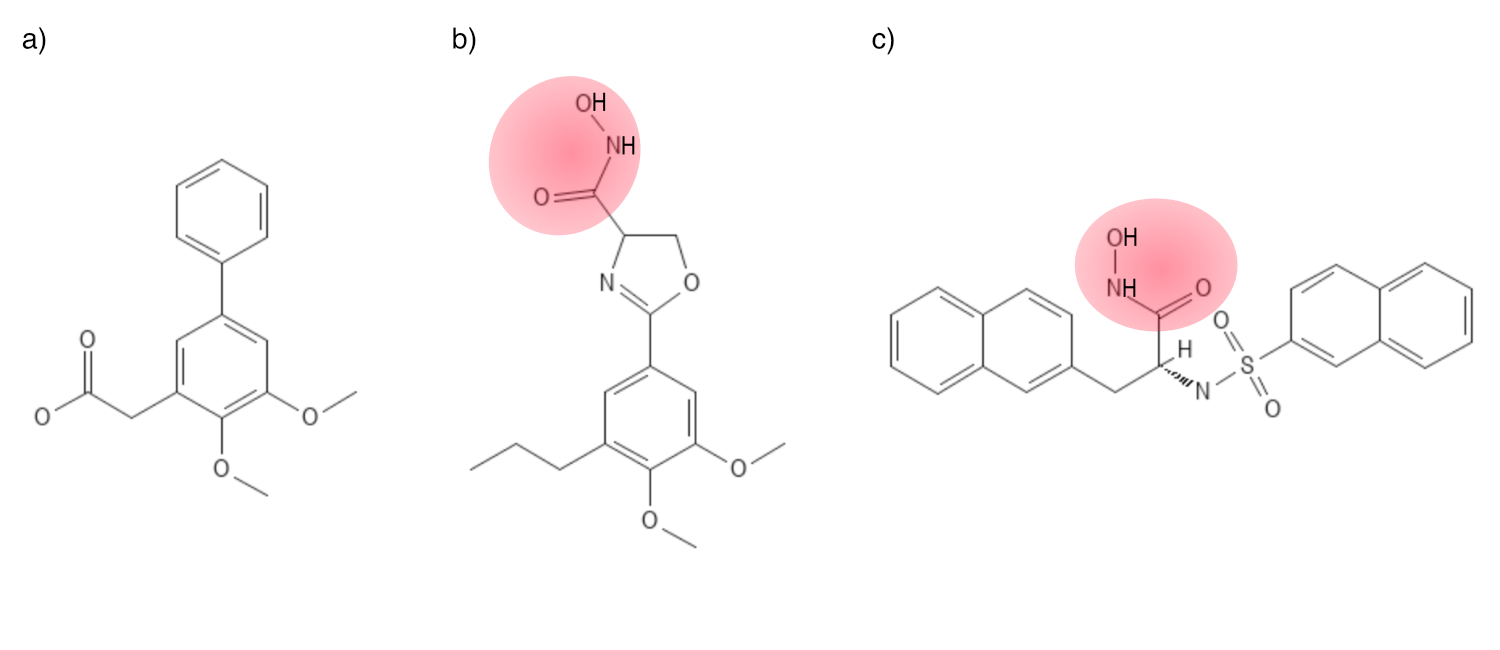
\includegraphics[width=1\textwidth]{imgs/results/compromise-molecule.png}
            \caption{(a) compromise solution, (b) similarity objective and (c) dissimilarity objective.}
        \end{figure}
    \end{columns}

\end{frame}


\begin{frame}{Results: molecular docking \hfill {\footnotesize \alert{DockTDesign}}}
    \begin{columns}[c]
        \column{.475\textwidth}
        \begin{block}{Protocol I}
            \textbf{Objectives}:
            \begin{itemize}
                \item[1.] maximize QED;
                \item[2.] minimize SA;
                \item[3.] minimize complexity;
                \item[4.] minimize binding affinity for LpxC;
                \item[5.] maximize binding affinity for MMP-9.
            \end{itemize}
        \end{block}

        \column{.475\textwidth}
        \begin{block}{Protocol II}
            \textbf{Objectives}:
            \begin{itemize}
                \item[1.] maximize QED;
                \item[2.] minimize binding affinity for LpxC;
                \item[3.] maximize binding affinity for MMP-9.
            \end{itemize}
            \textbf{Constraints}:
            \begin{itemize}
                \item[1.] SA less than or equal to 4;
                \item[2.] complexity between 150 and 600;
                \item[3.] molecular weight above 150 Da;
                \item[4.] QED above 0.5.
            \end{itemize}
        \end{block}
    \end{columns}
\end{frame}


\begin{frame}{Results: molecular docking (protocol I) \hfill {\footnotesize \alert{DockTDesign}}}
    \begin{figure}
        \centering
        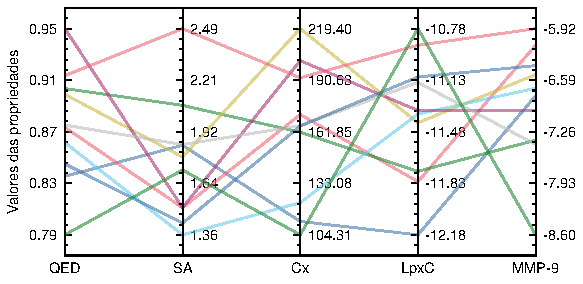
\includegraphics[width=.8\textwidth]{imgs/results/protocol1-parallel-coords}
        \caption{Parallel coordinates plot for the solutions obtained with protocol I.}
    \end{figure}
\end{frame}


% \begin{frame}{Resultados: atracamento molecular (protocolo I) \hfill {\footnotesize \alert{DockTDesign}}}
%     \begin{figure}
%         \centering
%         \includegraphics[width=1\textwidth]{imgs/results/protocol1-cmpds-h.pdf}
%         \caption{Dez primeiras soluções obtidas com o protocolo I.}
%     \end{figure}
% \end{frame}


\begin{frame}{Results: molecular docking (protocol II) \hfill {\footnotesize \alert{DockTDesign}}}
    \begin{figure}
        \centering
        \includegraphics[width=.8\textwidth]{imgs/results/protocol2-parallel-coords}
        \caption{Parallel coordinates plot for the solutions obtained with protocol II.}
    \end{figure}
\end{frame}

% \begin{frame}{Resultados: atracamento molecular (protocolo II) \hfill {\footnotesize \alert{DockTDesign}}}
%     \begin{figure}
%         \centering
%         \includegraphics[width=1\textwidth]{imgs/results/protocol2-cmpds-h.pdf}
%         \caption{Dez primeiras soluções obtidas com o protocolo II.}
%     \end{figure}
% \end{frame}


\begin{frame}{Results: molecular docking \hfill {\footnotesize \alert{DockTDesign}}}
    \begin{table}
        \centering
        \caption{Uniqueness metrics on the Pareto front, internal diversity (DivInt) and novelty considering the molecules generated by experimental protocols I and II.}
        \begin{tabular}{@{}llll@{}}
            \toprule
            Protocol & Uniqueness@FP  & DivInt         & Novelty        \\ \midrule
            I        & \textbf{0,920} & \textbf{0,745} & 0,653          \\
            II       & 0,825          & 0,451          & \textbf{0,915} \\ \bottomrule
        \end{tabular}
    \end{table}
\end{frame}



\begin{frame}{Results: molecular docking (protocol I) \hfill {\footnotesize \alert{DockTDesign}}}
    \begin{figure}
        \centering
        \includegraphics[width=1\textwidth]{imgs/results/figure-compound1-protocol1-h.png}
        \caption{Compound 1 from protocol I in the active sites of (a) LpxC and (b) MMP-9. LpxC: -12{,}176 kcal/mol; MMP-9: -6{,}795 kcal/mol; QED: 0{,}836; SA: 1{,}85; Cx: 111{,}781.}
    \end{figure}
\end{frame}


\begin{frame}{Results: molecular docking (protocol I) \hfill {\footnotesize \alert{DockTDesign}}}
    \begin{figure}
        \centering
        \includegraphics[width=1\textwidth]{imgs/results/figure-compound9-protocol1-h.png}
        \caption{Compound 9 from protocol I in the active sites of (a) LpxC and (b) MMP-9. LpxC: -10{,}897 kcal/mol; MMP-9: -5{,}924 kcal/mol; QED: 0{,}911; SA: 2{,}488; Cx: 191{,}971.}
    \end{figure}
\end{frame}


\begin{frame}{Results: molecular docking (protocol II) \hfill {\footnotesize \alert{DockTDesign}}}
    \begin{figure}
        \centering
        \includegraphics[width=1\textwidth]{imgs/results/figure_compound1_protocol2_h.png}
        \caption{Compound 1 from protocol II in the active sites of (a) LpxC and (b) MMP-9. LpxC: -13{,}331 kcal/mol; MMP-9: -7{,}801 kcal/mol; QED: 0{,}83; SA: 2{,}66; Cx: 247{,}997.}
    \end{figure}
\end{frame}


\begin{frame}{Results: molecular docking (protocol II) \hfill {\footnotesize \alert{DockTDesign}}}
    \begin{figure}
        \centering
        \includegraphics[width=1\textwidth]{imgs/results/figure-compound9-protocol2-h.png}
        \caption{Compound 9 from protocol II in the active sites of (a) LpxC and (b) MMP-9. LpxC: -11{,}794 kcal/mol; MMP-9: -4{,}694 kcal/mol; QED: 0{,}814; SA: 1{,}813; Cx: 178{,}732.}
    \end{figure}
\end{frame}

\section{Conclusions and Perspectives}


\begin{frame}{Conclusions \hfill {\footnotesize \alert{DockTDesign}}}

    \begin{itemize}
        \item Integration of \textbf{HierVAE} with \textit{many}-objective evolutionary algorithms presents itself as an effective and flexible approach.

              % \item NSGA-III outperforms NSGA-II and GA with aggregation in convergence and coverage of the Pareto front.

        \item NSGA-II generates molecules more diverse among themselves; NSGA-III explores innovative regions of chemical space. Adjustments in hyperparameters can improve both.

              % \item Predicted affinity and selectivity were optimized without dependence on structural similarity.

              % \item Treating SA and Cx as \textbf{constraints} (not objectives) improves predicted activity and selectivity.
        \item \textbf{DockTDesign}, together with \textbf{DockThor} and \textbf{DockTDeep}, presents itself as a promising and flexible platform for hit identification, capable of suggesting to the specialist a set of molecules that simultaneously meet multiple objectives.

    \end{itemize}

\end{frame}


% \begin{frame}{General conclusions}
%     \begin{itemize}
%         \item \textbf{DockTDeep} is a scoring function that is easy to train, robust to ligand/protein biases and rotational variance, and competitive with the state of the art in various evaluation scenarios.
%         \item \textbf{DockTDesign}, together with \textbf{DockThor} and \textbf{DockTDeep}, presents itself as a promising and flexible platform for hit identification, capable of suggesting to the specialist a set of molecules that simultaneously meet multiple objectives.
%     \end{itemize}
% \end{frame}



% \begin{frame}{Perspectives}

%     \begin{itemize}
%         \item Incorporate \textbf{DockTDeep} into the DockThor portal (\url{https://dockthor.lncc.br}).

%         \item Include multiple conformations (docking/molecular dynamics) to model \textbf{dynamic} aspects of binding.

%         \item Evaluate \textbf{DockTDeep} in \textit{lead} optimization tasks with experimental data and compare with FEP.

%         \item Use \textbf{metamodels} to reduce computational cost of docking in optimization.

%         \item Expand the approach to other therapeutic targets (including the multi-target scenario).

%         \item Collaborate with experimental groups to define realistic objectives and validate generated molecules.

%         \item Develop a \textbf{web portal} for the \textit{DockTDesign} platform, integrated with the Santos Dumont supercomputer.
%     \end{itemize}

% \end{frame}

%------------------------------------------------

\begin{frame}[allowframebreaks]{Referências}
    \footnotesize
    % Override the bibliography template to show numbers
    % \setbeamertemplate{bibliography item}[text]
    \nocite{*} % Include all entries from the bib file
    \bibliography{reference.bib}
    \bibliographystyle{unsrt}
\end{frame}

%------------------------------------------------



\begin{frame}
    \Huge{\centerline{\textbf{Thank you!}}}
    \vspace{1em}
    % put logos, side by sides, for all these [imgs/logos/]: lncc-logo.png, logo-capes.png, logo-faperj.jpg, logo-sinapad.png
    \begin{center}
        \includegraphics[height=1.cm]{imgs/logos/lncc-logo.png}%
        \hspace{0.5cm}%
        \includegraphics[height=1.cm]{imgs/logos/logo-sinapad.png}
        \hspace{0.5cm}%
        \includegraphics[height=1.cm]{imgs/logos/logo-capes.png}%
        \hspace{0.5cm}%
        \includegraphics[height=1.cm]{imgs/logos/logo-faperj.jpg}%

    \end{center}
\end{frame}

%----------------------------------------------------------------------------------------


\begin{frame}{NSGA-II}
    \begin{columns}[c]
        \column{.475\textwidth}
        \begin{figure}
            \centering
            \includegraphics[width=1\textwidth]{imgs/nsga-ii.png}
            \caption{NSGA-II algorithm.}
        \end{figure}

        \column{.475\textwidth}
        \begin{figure}
            \centering
            \includegraphics[width=0.75\linewidth]{imgs/crowding-distance.png}
            \caption{Crowding distance in NSGA-II.}
        \end{figure}
    \end{columns}
\end{frame}


\begin{frame}{NSGA-III: reference directions}
    \begin{figure}
        \centering
        \includegraphics[width=.4\textwidth]{imgs/nsgaiii-crowding.png}
        \caption{Reference directions in NSGA-III.}
    \end{figure}

\end{frame}


\begin{frame}
    \includegraphics[width=1\textwidth]{imgs/extras-1.png}
\end{frame}


\begin{frame}
    \includegraphics[width=1\textwidth]{imgs/extras-2.png}
\end{frame}


\begin{frame}
    \includegraphics[width=1\textwidth]{imgs/extras-3.png}
\end{frame}

\end{document}